%%%%%%%%%%%%%%%%%%%%%%%%%%%%%%%%%%%%%%%%%
% Imperial Placement Report Template 
% LaTeX Template
% Version 1.0 (28/09/16)
%%%%%%%%%%%%%%%%%%%%%%%%%%%%%%%%%%%%%%%%%
%----------------------------------------------------------------------------------------
%	PACKAGES AND OTHER DOCUMENT CONFIGURATIONS
%----------------------------------------------------------------------------------------

\documentclass[12pt]{article}
\usepackage[english]{babel}
\usepackage[utf8x]{inputenc}
\usepackage{amsmath}
\usepackage{graphicx}
\usepackage[colorinlistoftodos]{todonotes}
\usepackage[toc,page]{appendix}
\usepackage{natbib}
\usepackage{tabularray}
\usepackage{caption}
\usepackage{amsmath}
\usepackage{float}
\usepackage{setspace}
\usepackage{caption}
\usepackage[abs]{overpic}
\usepackage{subcaption}


\DeclareCaptionFormat{myformat}{\fontsize{10}{12}\selectfont\textbf{#1#2}#3}
\captionsetup[figure]{format=myformat, labelsep=period}
\graphicspath{{figures/}}


\onehalfspacing
\begin{document}

\begin{titlepage}

\newcommand{\HRule}{\rule{\linewidth}{0.5mm}} % Defines a new command for the horizontal lines, change thickness here
\setlength{\topmargin}{0in}
\center % Center everything on the page
 
 
 \begin{minipage}{0.4\textwidth}
\begin{flushleft} \large
\hspace*{-0.5cm}
\includegraphics[scale=0.14]{figures/imperial.png}\\
\end{flushleft}
\end{minipage}
~
\begin{minipage}{0.5\textwidth}
\begin{flushright} \large
\hspace*{2cm}
\end{flushright}
\end{minipage}\\[1cm]
%----------------------------------------------------------------------------------------
%	HEADING SECTIONS
%----------------------------------------------------------------------------------------

\textsc{\LARGE Imperial College of Science, Technology and Medicine}\\[1.2cm] % Name of your university/college
\textsc{\Large Department of Life Science}\\[0.4cm] % Major heading such as course name
\textsc{\large MSc Computational Methods in Ecology and Evolution}\\[0.4cm] % Minor heading such as course title

%----------------------------------------------------------------------------------------
%	TITLE SECTION
%----------------------------------------------------------------------------------------

\HRule \\[0.4cm]
{ \huge \bfseries Using genetic frequency time-series to detect sites under selection}\\[0.4cm] % Title of your document
\HRule \\[0.4cm]
 
%----------------------------------------------------------------------------------------
%	AUTHOR SECTION
%----------------------------------------------------------------------------------------

\begin{minipage}{0.4\textwidth}
\begin{flushleft} \large
\emph{Author:}\\
Chuxinyao \textsc{Wang} \\ % Your name

\emph{CID:}\\
02248307
\end{flushleft}
\end{minipage}
~
\begin{minipage}{0.5\textwidth}
\begin{flushright} \large
\emph{Supervisor:} \\
Dr. Bhavin \textsc{Khatri} \\[0.5cm] % Supervisor's Name
\end{flushright}
\end{minipage}\\[1cm]

%----------------------------------------------------------------------------------------
%	DATE SECTION
%----------------------------------------------------------------------------------------

{\large August 2023}\\[0.5cm] % Date, change the \today to a set date if you want to be precise
A thesis submitted in partial fulfilment of the requirements for the degree of
Master of Science/Research at Imperial College London
Submitted for the MSc in Computational Methods in Ecology and Evolution

\vfill % Fill the rest of the page with whitespace
\newpage
Declaration\\
The actual data for this study came from Prof. Nastoulli of UCL Hospital (UCLH). The simulated data for this study was coded and implemented by myself. In addition, part of the code for parameter optimisation and multi-hypothesis testing analysis was written and provided by Dr. Khatri. The analysis of the data was completed by myself under the guidance of Dr. Khatri. The simulations and data analysis for this study involves large computation, so high-performance computing were required for most of the work. Regarding the availability of the code, since the code of the analysis part is still in the testing stage and the ownership belongs to Dr. Khatri Bhavin, it cannot be made public. Please contact Dr. Khatri Bhavin if necessary. For the part of simulation generating frequency data, please email the author himself.
\vfill
\end{titlepage}


\renewcommand{\abstractname}{Abstract}

\begin{abstract}
The Wright-Fisher(WF) model is a discrete-time method for describing the evolution of populations. Under the framework of the WF model, this study uses an approximate solution of the stochastically change of gene frequency to evaluate its feasibility of inferring the evolution of virus populations in nature. Here, we conduct simulations of single site analysis and genome wide analysis. Single site analysis is to test the ability of such method to characterise optimum parameters. And genome wide analysis is to evaluate feasibility in detecting selection sites in genes under likelihood estimation method as well as the statistical analysis of multi-hypothesis. We apply this method to two intrahost datasets of immunocompromised patients infected with SARS-CoV-2, then interpret the results in light of the simulation analysis. However, we noticed that different parameter constrained situations can affect the accuracy of detecting selection.

\end{abstract}

\newpage
\tableofcontents

\newpage

\section{Introduction}
The time series of allele frequencies is of great help in many studies in the field of population genetics and evolution \citep{bollback2008estimation}, such as human ancient DNA (aDNA) data \citep{hummel2005detection}, virus population data\citep{shankarappa1999consistent}, and experimental evolutionary population data (drosophila, bacteria, phage) \citep{buri1956gene, woods2006tests, bollback2007clonal}. This is because the strength of selection and the anticipated change in allele frequency over time are closely related \citep{bollback2008estimation}. Current methods for detecting genetic selection in evolution heavily rely on the analysis of synonymous and nonsynonymous substitutions ratio ($dN/dS$). Despite the established utility of the $dN/dS$ ratio in comparing evolutionary processes among different independent populations, its application to gene sequences within a single population has shown reduced sensitivity in detecting natural selection \citep{kryazhimskiy2008population}. Hence, $dN/dS$ is not applicable for the study of segregating variation in a population. Although time-series methods for detecting selection of single site exist and are popular \citep{bollback2008estimation, malaspinas2012estimating, tataru2015inference}, a genome wide selection analysis is still computationally expensive \cite{khatri2016quantifying}. Whereas, an analytical stochastic dynamics solution would have the significant advantage of directly evaluating the likelihood function, allowing for very efficient computation of the maximum likelihood estimation for parameter optimisation \citep{khatri2016quantifying}. An analytical solution was developed by Khatri (2016) which can use gene frequency data changes over time can explore the impact of three genetic pressures (genetic drift, selection and mutation) on species population evolution. This study will evaluate the use of this method on estimating parameters and detecting selection in evolution at both genome-wide level and single site level.\\

Despite the fact that the method of estimating the selection coefficient of a single genetic locus from time-series data has been extensively used in the study of the evolution of simple traits \citep{jewett2016effects}, for the evolution of viruses, such as RNA virus, due to its high variability, high mutation rate, and low virus replication cycle characteristics \citep{domingo1996basic}, their evolutionary history are more difficult to determine from direct observation of phenotypic changes. Therefore, it is considered here that starting from the genotype of the virus, the evolution of the virus can be directly obtained through the changes in the nucleotides at the locus on the sequence. Hypothesis testing for an entire gene sequence presents another problem, increasing the number of Type 1 errors \citep{goeman2014multiple}. If only two entire gene sequences are compared for hypothesis testing, there might be about 500 sites occur Type I error on the gene sequence if $\alpha =0.05$, $L= 10,000$ number of locus, which is unacceptable. Therefore, this study will also use the method of multi-hypothesis testing to verify and compare the evolution results in sequences to reduce Type I error.\\

In this study we simulate gene frequency change time series using the Wright-Fisher genetic model under conditions of genetic drift, selection and mutation, assuming two variant possibilities (wild-type and mutant). The three parameters of $N$, $\mu$ and $s$ are estimated by Maximum Likelihood Estimation (MLE), and p-values calculated by the Likelihood Ratio Test (LRT) used as a decision statistic for multi-hypothesis testing from simulated genome wide data. Finally, the Receiver Operating Characteristic (ROC) curve \citep{zweig1993receiver} is used to obtain Area Under the ROC Curve(AUC) to test the performance of multi-hypothesis testing. In addition, the study also used the real data of SARS-CoV-2 patients to verify the accuracy of the method, and explored the evolved loci differences in virus gene sequence in patients with immunocompromised \citep{choi2020persistence, clark2021sars, markov2023evolution} infection, specifically, locate locus under selection from virus intra-host evolution.\\

%**********************************************%
\newpage
\section{Methods}
\subsection{Use and implementation of mathematical methods}
The study adopts the WF model and considers the effects of genetic drift, selection, and mutation in haploid RNA viruses (SARS-CoV-2 in this study) with $N$ individuals, consider the wild type and mutant ($N-n$) individuals ($n$). Genetic drift refers to the process of random changes in gene frequency due to the influence of random events in a finite population. This change is caused by random factors, and the effect is more significant in small populations. Genetic drift can be simplest described as binomial sampling in WF model, which is half the variance of the variation frequency between generations (\textbf{Eqn.1}) \citep{kimura1983neutral}. Selection refers to the variation of gene frequency caused by the adaptive difference among individuals in nature, which can be favorable adaptation or unfavorable adaptation. In addition, mutations refer to random, heritable changes that occur in a gene or genome, and also has forward and backward mutations. Expressed in discrete form is \textbf{Eqn. 2}. It represents the average change in mutation frequency per generation due to selection and mutation. Where $s$ is the selection coefficient. If it is a preference choice from the wild type to the mutant type, then $s>0$ means positive selection, otherwise $s<0$ means negative selection. $\mu_1$ is the forward mutation coefficient, indicating the mutation rate from wild type to mutant type, and vice versa, the backward mutation rate from mutant type to wild type is $\mu_2$. 

\begin{align}
  &  D(x) = \frac{x(1-x)}{2N}\\
  &  M(x) = sx(1-x) + \mu_1(1-x) + \mu_2 x 
\end{align}

    \textbf{Eqn. 3 and 4} are coded in MATLAB to simulate genetic pressure. Let $n(t)$ be the number of mutant type in generation $t$ and $x(t)={n(t)}/{N}$ be the corresponding frequency of mutant type. The random mating of the population leads to a count of wild type in generation $t+1$ that is binomial distributed (Eqn.6) \citep{wright1931evolution, crow1970introduction, fisher1999genetical, ewens2004mathematical}. Therefore, $n(t+1)/N$ is the frequency of the variant in generation $t+1$ (Eqn.7). This enables the implementation of random drift changes into computer simulations.

\begin{align}
  &  \frac{\delta x} {\delta t} = M(x)\\
  &  \delta x = M(x) \delta t\\
  &  n(t+1)∣n(t)∼Bin(N,x(t)+ \delta x) \\
  &  x(t+1) = \frac{n(t+1)∣n(t)∼Bin(N,x(t)+ \delta x)} {N}
\end{align}


Besides, $M(x)$ (Eqn.2) can be used to simulate the impact of selection and mutation on gene frequency on computer.Yet positive selection and negative selection are categorised and used in this study because this research covered both of these types of selection. WF model was run in MATLAB in discrete time to perform independent simulations for each site (assuming that each site in the genome evolves independently). Simulate actual sampling by controlling the sampling time interval. As a result, a set of matrix f (number of time sites, length of the genome) will be obtained to store the sampling time ($t$), and the frequency of the mutant gene in the population corresponding to the time ($x(t)$) to evaluate the accuracy of the maximum likelihood parameter estimation .\\
\subsection{Single site Monte-Carlo simulation with selection, mutation and genetic drift under Wright-Fisher model} 

Setting initial parameters, timescales and frequencies of the simulated data are based on the establishment of mutants proposed by \cite{desai2007beneficial}. Establishment describes a beneficial mutant needs to survive and overcome genetic drift to reach certain frequency before fixing, that frequency is established frequency. For positive selection, especially the selection advantage ($2Ns>>1$), according to \cite{desai2007beneficial}, there is an average frequency ($1/2Ns$) for mutants to establish. Before this frequency is reached, mutants increases in specific rate to reach the establishment as soon as possible, it takes around $\tau_{est}= \frac{\ln 2}{s} >\frac{1}{2s}$. Once reached, it will increase at an exponential rate until it is fixed. Therefore the total mean time to fixation from zero frequency can be calculated by \textbf{Eqn. 7} \citep{desai2007beneficial}. \\

For negative selection, there is mutation selection balance \citep{crow1970introduction}. Mutation-selection balance refers to a situation in which the rate at which new deleterious mutations are introduced into a population is balanced by the rate at which they are removed through selection. By using \textbf{Eqn. 2}, equilibrium can be found, which is $x_{eqm}=\frac{\mu}{|s|}$ when ($\mu=\mu_1=\mu_2$), and time to reach the equilibrium is $\tau_{eqm} =\frac{1}{|s|}$.\\
\begin{align}
  &  \tau_{fix} =\frac{1}{2s}\times(1+\ln(Ns))
\end{align}


In order to match virus data situation \citep{seo2002estimation, sanjuan2010viral}, $N\mu$ is set to 1 here, that is, the population size $N=10000$, the mutation rate $\mu=10^{-4}$.\\

We choose a selection coefficient $s=0.005$ for positive selection, which gives a mean time to fixation of $\tau\approx261$ generations. \\

We choose $T=10000$ much greater than $\tau$ for simulations under positive selection in this single-gene simulation, and with $\Delta\ t=\{10,20,30,40,50,100$ $,150,200,300,400,500\}$ $(\tau\approx1/2s=100\ generations)$. Then, in order to explore the impact of stopping the simulation at fixation on parameter estimation, we cut off the simulation once if fixed to increase estimation accuracy.\\

In order to explore the influence on the selection coefficient estimation before and after the establishment, we set part of the initial frequencies below the establishment frequency and part above the establishment frequency (the establishment frequency is about $1/2Ns=0.01$, $x_0=\left\{0, 0.001, 0.01, 0.1, 0.5\right\}$.\\

For negative selection, $s$ is set to $-0.005$ the initial frequency is set to the mean frequency $x_0=\frac{\mu}{|s|}=0.002$ in mutation-selection balance, which can be obtained from \textbf{Eqn. 1}. Same $T$ and $\Delta t$ are chosen for negative selection too. Whole single site simulation use Monte Carlo simulation to perform 500 simulations. The median value of the optimised parameters obtained by MLE is compared with the initial parameters in the range $log_{10}$.\\


\subsection{Genome-wide simulation with selection, mutation and genetic drift under Wright-Fisher model}  

Genome wide simulations used the WF model with selection, mutation and genetic drift, including parameters population size ( $N$ ), positive and negative selection coefficient ($s_{pos} > 0$, $s_{neg} < 0$), mutation rate ($\mu$), fraction of negative selection sites in the genome ($fr$), initial frequency distribution ($x(0)$), total number of generations ( $T$ ), sampling time interval ( $\Delta t$ ), and genome length ($L$). Besides, sample by binomial distribution (\textbf{Eqn. 8}) to simulate read-depth, and the number of reads is $ns=100$.
\begin{align}
  & x_{sampled}(i,k) = \frac{Bin(ns,X(i,k)}{ns}
\end{align}
We assume that the initial frequency is derived from a balanced distribution of allele frequencies in mutation-selection balance. When $s<0$ and $2N|s|>>1$ (Selective advantage) \citep{desai2007beneficial} this is approximately a gamma distribution ($shape=2N\mu$, $scale=2N|s|$) \citep{kim2017inference}. For the initial frequency of the genome sites subject to positive selection, random sampling in the interval $[0, 1]$ is used to generate it. $fr$ is 0.8 (in the case of $L=10000$ genomic positions, the number of negative selection sites is 8000). \\

In addition, according to \cite{10.1093/genetics/47.6.713}, the value of $2N|s|$ that mutation will be under strong selection among population ($2Ns >1$ or $2N|s| <-1$ or neutral ($0<2N|s|<1$). Because of this, we assume an exponential Distribution fitness effect (DFE). DFE is a concept in genetics that describes the proportion of new mutations that are beneficial, neutral, or deleterious \citep{eyre2007distribution}. Note that for the fraction of neutral mutations in an exponential DFE is a simplification and approximation that holds under our assumptions which can be calculated by $\frac{1}{2N}=5\times 10^{-5}$ \citep{kimura1979model},so sites with $s\leq 10^{-5}$ is effectively neutral.  When a fraction of sites in the genome are effectively neutral, it means that mutations occurring at those sites have minimal impact on an individual's fitness.\\

Based on the above, the simulation tests the impact of different possibilities of $T$ and $\Delta t$ on parameter estimation, and evaluate their performance through the ROC and AUC. For total iterative generations, there are $T=\{1000,10000\}$. When $T=1000$, $\Delta t$ is set to ${5, 10, 20, 50}$, when $T=10000$, $\Delta t$ is set to $\{50, 100, 200, 500\}$.This is because under positive selection, more than generation of establishment time $\tau_{est}= \frac{\ln 2}{s} >\frac{1}{2s}$ can better observe the fixation of mutant \citep{desai2007beneficial}. So $s_{pos}$ is set to $0.005$ ($\tau_{est}=100$ in this case). Besides, amount of sequences in this study is set to $N=10000$, $\mu$ is $10^{-5}$, satisfying $N\mu=0.1$, and $s_{neg}$ is set to $2 \times 10^{-4}$. The mutant gene frequencies of the whole population are stored in a matrix generated under different regimes. All matrices are executed through a set of purpose-built MATLAB programs, which contain the frequency change of each polymorphic site at time T. In order to explore the impact of sampling on the parameter estimations, simulations are also divided into two groups, one group is the result with binomial sampling as mentioned before, and the other group is the result without binomial sampling. The above simulation results are saved and used for further analysis in  subsequent MLE parameter estimation and multi-hypothesis testing (see subsection 2.4 for details).\\




\subsection{SARS-CoV-2 patient data processing and analysis} 
The patient data from March 2020 to February 2021 provided by Prof. Nastoulli of UCL Hospital (UCLH) are used in this study. Using the iVar tool, the data is transformed from the $bam$ file format into a $tsv$ file \citep{danecek2011variant}. Single nucleotide variants (SNVs) and indels are called using the output of the command by iVar \citep{grubaugh2019amplicon}. Each $tsv$ file represents the gene frequency of the virus in a patient's host on a test date. By combining multiple $tsvs$, a list of SARS-CoV-2 virus nucleotide frequency records over time can be obtained. This is pre-processed to converted to '.mat' format by Dr. Khatri. And data named 'Patient 6' and 'Patient 9' are used for the analysis of this study.  For each patient, 3 '.mat' files are stored. Respectively, an frequency array $f(i, j, k)$, $i$ represents the gene frequency. The number of $i$ should be 29903 nucleotides \citep{wu2020new} for SARS-CoV-2; $j$ represents the type of variation, including six types: A, T, C, G ,insertion and deletion; $k$ represents the patient disease time, which can be used to express the time scale of frequency changes. Besides, an array $dparray(i,k)$ records read-depth \citep{grubaugh2019amplicon} of each nucleotide of each patient at each recorded date. So $I$ has 29903 rows ($i$) and number of dates recorded column ($k$).And $t$ array indicates the number of days since positive. The above arrays are saved and used for further analysis in the MATLAB function written for subsequent MLE parameter estimation and multi-hypothesis testing (see the next subsection for details).\\




\vfill
\subsection{Parameter Optimisation based on MLE and Implementation of Multi-hypothesis Testing} 

The analysis of the simulated data in the above subsections and the analysis of the patient data are estimated by using MLE to obtain the optimised parameters. The MLE equation was written by Dr. Khatri and provided for use in this study. The function computes the best $N$, $\mu$, and $s$ ($Nopt, muopt, sopt$) for each site and uses maximum likelihood to evaluate whether site-based selection is effective. For the data of whole gene, no matter simulated and real data, the above function is executed through loops to optimise the parameters of each gene site in turn, and finally gather three lists corresponding to the three parameters. The 'Simplex' optimisation method is used for likelihood estimation which developed by \cite{nelder1965simplex}. In the case of optimising three parameters at the same time, the function can also draw the likelihood surface for each estimate, including the 95$\%$ confidence surface. Furthermore, in order to find a better regime, i.e., what condition has the least difference for parameter estimation. This study also discusses the situation of fixing $N$ and $\mu$. In general, there are: 1. Optimising three parameters at the same time; 2. Fixing $N$ to optimise $\mu$ and $s$, 3. Fixing $\mu$ to optimise $N$ and $s$; 4. Both $N$ and $\mu$ are fixed to optimise $s$. This is a classified discussion made to explore the relationship between virus evolution within a host and evolution between hosts under selection with real data. \\

For the analysis of multiple hypothesis testing, simulated data and real data are different. First, the simulation of a single site does not require this part of the analysis. The parameter optimisation results of whole genome simulation under different regimes are used for ROC drawing and AUC value. We plot false discoveries vs true discoveries for all sites ordered by the LRT statistic with the largest first on ROC. AUC is the area under this curve and the larger AUC the better the performance calculation through Likelihood Ratio Statistic ($d_0 = 2\times(\ln(L_{max})-\ln(L_{max0}))$) as a statistical decision, where $L_{max}$ indicates the maximum likelihood function value and $L_{max0}$ indicates the maximum likelihood function value of the null model (s=0). A perfect ROC curve would have a vertical line from the origin to $TPR = 1$, indicating that all selected sites were detected correctly, followed by a horizontal line $FPR=1$, indicating all neutrally evolved sites. 'perfcurve' in MATLAB can accomplish this purpose. \citep{fawcett2004roc}. Among them, the labels are classified according to whether $2Ns>1$, that is, whether the site is neutral or under selected. The classification score is list $d_0$, and 1 represents the positive class. The obtained AUC values are classified according to different regimes, and line charts of AUC changes are drawn.\\

Multi-hypothesis testing analysis for real data uses the Benjamini-Hochberg (BH) false discovery rate controling method \citep{benjamini1995controlling}. BH method finds all discoveries with False Discovery Rate(FDR) $\textless 0.05$ to sort the $p-value$ and  $q-value$ stated by \cite{storey2002direct} is roughly the FDR for each site . $q-value$ is calculated by built-in function 'mafdr' \citep{storey2004strong, storey2003positive,  storey2003statistical}. The $q-value$ is used as the score in the ROC. The label is assigned according to $p-value$. The $p-value$ is obtained from the value of the complement of the chi-square cumulative density function ('chi2cdf' in MATLAB) with the difference $n$ between the number of degrees of freedom of full model vs null model  calculated at the value in $d_0$ \citep{abramowitz1968handbook}. The code implementation of this part is done by Dr. Khatri.

%**********************************************%

\newpage
\section{Results}
\subsection{Single site parameter estimation results}
First look at the positive selection part of the single site simulation. \textbf{Figure 2-4} show the error changing of assessing parameter estimating accuracy on a $log_{10}$ of magnitude scale between the optimised parameter value and the set parameter value under different $\Delta t$ for 4 different parameter fixing conditions. For $s$ (\textbf{Figure. 1}), the situation is simple. As $\Delta t$ increases, the error between the estimated value and the initial set value gradually decreases, forming an reverse exponential downward trend. However, it is worth noting that the error at $x_0=0.5$ has a significant error compared with other initial frequencies. The error is about 0.5 orders of magnitude higher than other initial frequencies.\\

For $N$ (\textbf{Figure. 2}), as $\Delta t$ increases, the error from the initial $N$ value gradually decreases, and the smallest error occurs in the simulation of $\Delta t=40$ with a error of less than 0.2 log 10 scale, and then as $\Delta t $ increases, the error gradually increases again. Especially for the simulation of $x_0=0.5$, the error at $\Delta t=500$ has a large gap compared to other initial frequency cases. Overall, the error between optimising the three parameters at the same time is smaller than when $\mu$ is fixed.\\

For $\mu$ (\textbf{Figure. 3}), the situation is similar to $N$, the smallest error occurs at $\Delta t=50$, and the error gradually increases after $\Delta t=50$. Unlike the error of $N$, the maximum error of $\mu$ is always no greater than 0.8.


\begin{figure}[H]
    \centering
    \hspace{-1cm}
    \makebox[\textwidth][c]{\includegraphics[width=1.3\textwidth,height=0.4\textheight]{figures/opt/sampled_diff_s.eps}}
    \put(0,0){\textcolor{black}{\textbf{A}}}
    \label{fig:pt6_pvalue}
\end{figure}

\begin{figure}[H]
    \centering
    \hspace{-1cm}
    \makebox[\textwidth][c]{\includegraphics[width=1.3\textwidth,height=0.4\textheight]{figures/fixN/sampled_diff_s.eps}}
    \put(0,0){\textcolor{black}{\textbf{B}}}
    \label{fig:pt6_pvalue}
\end{figure}

\begin{figure}[H]
    \centering
    \hspace{-1cm}
    \makebox[\textwidth][c]{\includegraphics[width=1.3\textwidth,height=0.4\textheight]{figures/fixmu/sampled_diff_s.eps}}
    \put(0,0){\textcolor{black}{\textbf{C}}}
    \label{fig:pt6_pvalue}
\end{figure}

\begin{figure}[H]
    \centering
    \hspace{-1cm}
    \makebox[\textwidth][c]{\includegraphics[width=1.3\textwidth,height=0.4\textheight]{figures/fixNmu/sampled_diff_s.eps}}
    \put(0,0){\textcolor{black}{\textbf{D}}}
    \caption{\textbf{$s$ error for single site positive selection simulation.} A is result by optimising $N \mu s$, B is result by fixing $N$, C is result by fixing $\mu$ and D is result by fixing $N\ \mu$. Different colours indicates different initial frequencies.}
    \label{fig:pt6_pvalue}
\end{figure}

\begin{figure}[H]
    \centering
    \hspace{-1cm}
    \makebox[\textwidth][c]{\includegraphics[width=1.3\textwidth,height=0.4\textheight]{figures/opt/sampled_diff_N.eps}}
    \put(0,0){\textcolor{black}{\textbf{A}}}

    \label{fig:pt6_pvalue}
\end{figure}

\begin{figure}[H]
    \centering
    \hspace{-1cm}
    \makebox[\textwidth][c]{\includegraphics[width=1.3\textwidth,height=0.4\textheight]{figures/fixmu/sampled_diff_N.eps}}
    \put(0,0){\textcolor{black}{\textbf{B}}}
    \caption{\textbf{$N$ error for single site positive selection simulation.} A is result by optimising $N \mu s$, and B is result by fixing $\mu$. Different colours indicates different initial frequencies.}
    \label{fig:pt6_pvalue}
\end{figure}

\begin{figure}[H]
    \centering
    \hspace{-1cm}
    \makebox[\textwidth][c]{\includegraphics[width=1.3\textwidth,height=0.41\textheight]{figures/opt/sampled_diff_mu.eps}}
    \put(0,0){\textcolor{black}{\textbf{A}}}

    \label{fig:pt6_pvalue}
\end{figure}

\begin{figure}[H]
    \centering
    \hspace{-1cm}
    \makebox[\textwidth][c]{\includegraphics[width=1.3\textwidth,height=0.41\textheight]{figures/fixN/sampled_diff_mu.eps}}
    \put(0,0){\textcolor{black}{\textbf{B}}}
    \caption{\textbf{$\mu$ error for single site positive selection simulation.} A is result by optimising $N \mu s$, and B is result by fixing $N$. Different colours indicates different initial frequencies.}
    \label{fig:pt6_pvalue}
\end{figure}
For results in single site negative selection simulation (\textbf{Figure. 4}), result is roughly the same trend with positive selection in error of true $s$ and estimated $s$ decreases with the increase of $\Delta t$, but the error is larger than the result of positive selection. But the result of fixing $N$ when $\Delta t=200$ and later, the error is again gradually increased. However, $N$ error are different from situation in positive selection. When $\Delta t$ from 20 to 30, error unexpectedly increases in fixing $\mu$ condition. Then sharply decreases until $\Delta t=100$. Besides, in optimising three parameters condition, the error of $N$ doesn't change a lot at first 4 sampling time sites. Overall, the error in the optimization parameter $N$ under negative selection is still greater than that under positive selection. Finally, looking at $\mu$, the overall trend first increases and then decreases, which is similar to that of positive selection. It's just that the inflection point appears later, and there is an upward trend after $\Delta t=100$, and it is when $\Delta t=50$ under positive selection. \\

After comparing the errors of the real and estimated values of the parameters under positive selection and negative selection, it can be found that there are some differences in the estimated coefficients of different selections. For the estimation of $s$, the error between true value and estimated values under the positive selection is slightly lower than  under the negative selection. This shows that for the estimation of $s$, estimating the positive selection coefficient ($s\textless0$) is more accurate than the negative selection coefficient ($s\textless0$). Under each same sampling interval, the estimation error of positive selection on $s$ is about 0.2-0.6 order of magnitude smaller than that of negative selection. For the estimation of $N$, error between positive and negative selection is greater. The error range is about 0.2-1.2 orders of magnitude under positive selection, and 0.5-3 orders of magnitude under negative selection. For the estimation of $\mu$, the error difference between positive and negative selection is not big, which is reflected in the larger sampling interval, the negative selection has a larger error in the estimation of μ than the positive selection.\\


It is worth noting that all error lines that optimising three parameters lack the result of $\Delta t=400,500$. This is because the time series analysis here cannot be completed as expected, so there are not result.\\

\begin{figure}[H]
    \centering
    \hspace{-1cm}
    \makebox[\textwidth][c]{\includegraphics[width=1.6\textwidth,height=0.4\textheight]{figures/s_neg.eps}}
    \put(10,0){\textcolor{black}{\textbf{A}}}
    \label{fig:pt6_pvalue}
\end{figure}

\begin{figure}[H]
    \centering
    \hspace{-1cm}
    \makebox[\textwidth][c]{\includegraphics[width=1.6\textwidth,height=0.4\textheight]{figures/N_neg.eps}}
        \put(10,0){\textcolor{black}{\textbf{B}}}
    \label{fig:pt6_pvalue}
\end{figure}

\begin{figure}[H]
    \centering
    \hspace{-1cm}
    \makebox[\textwidth][c]{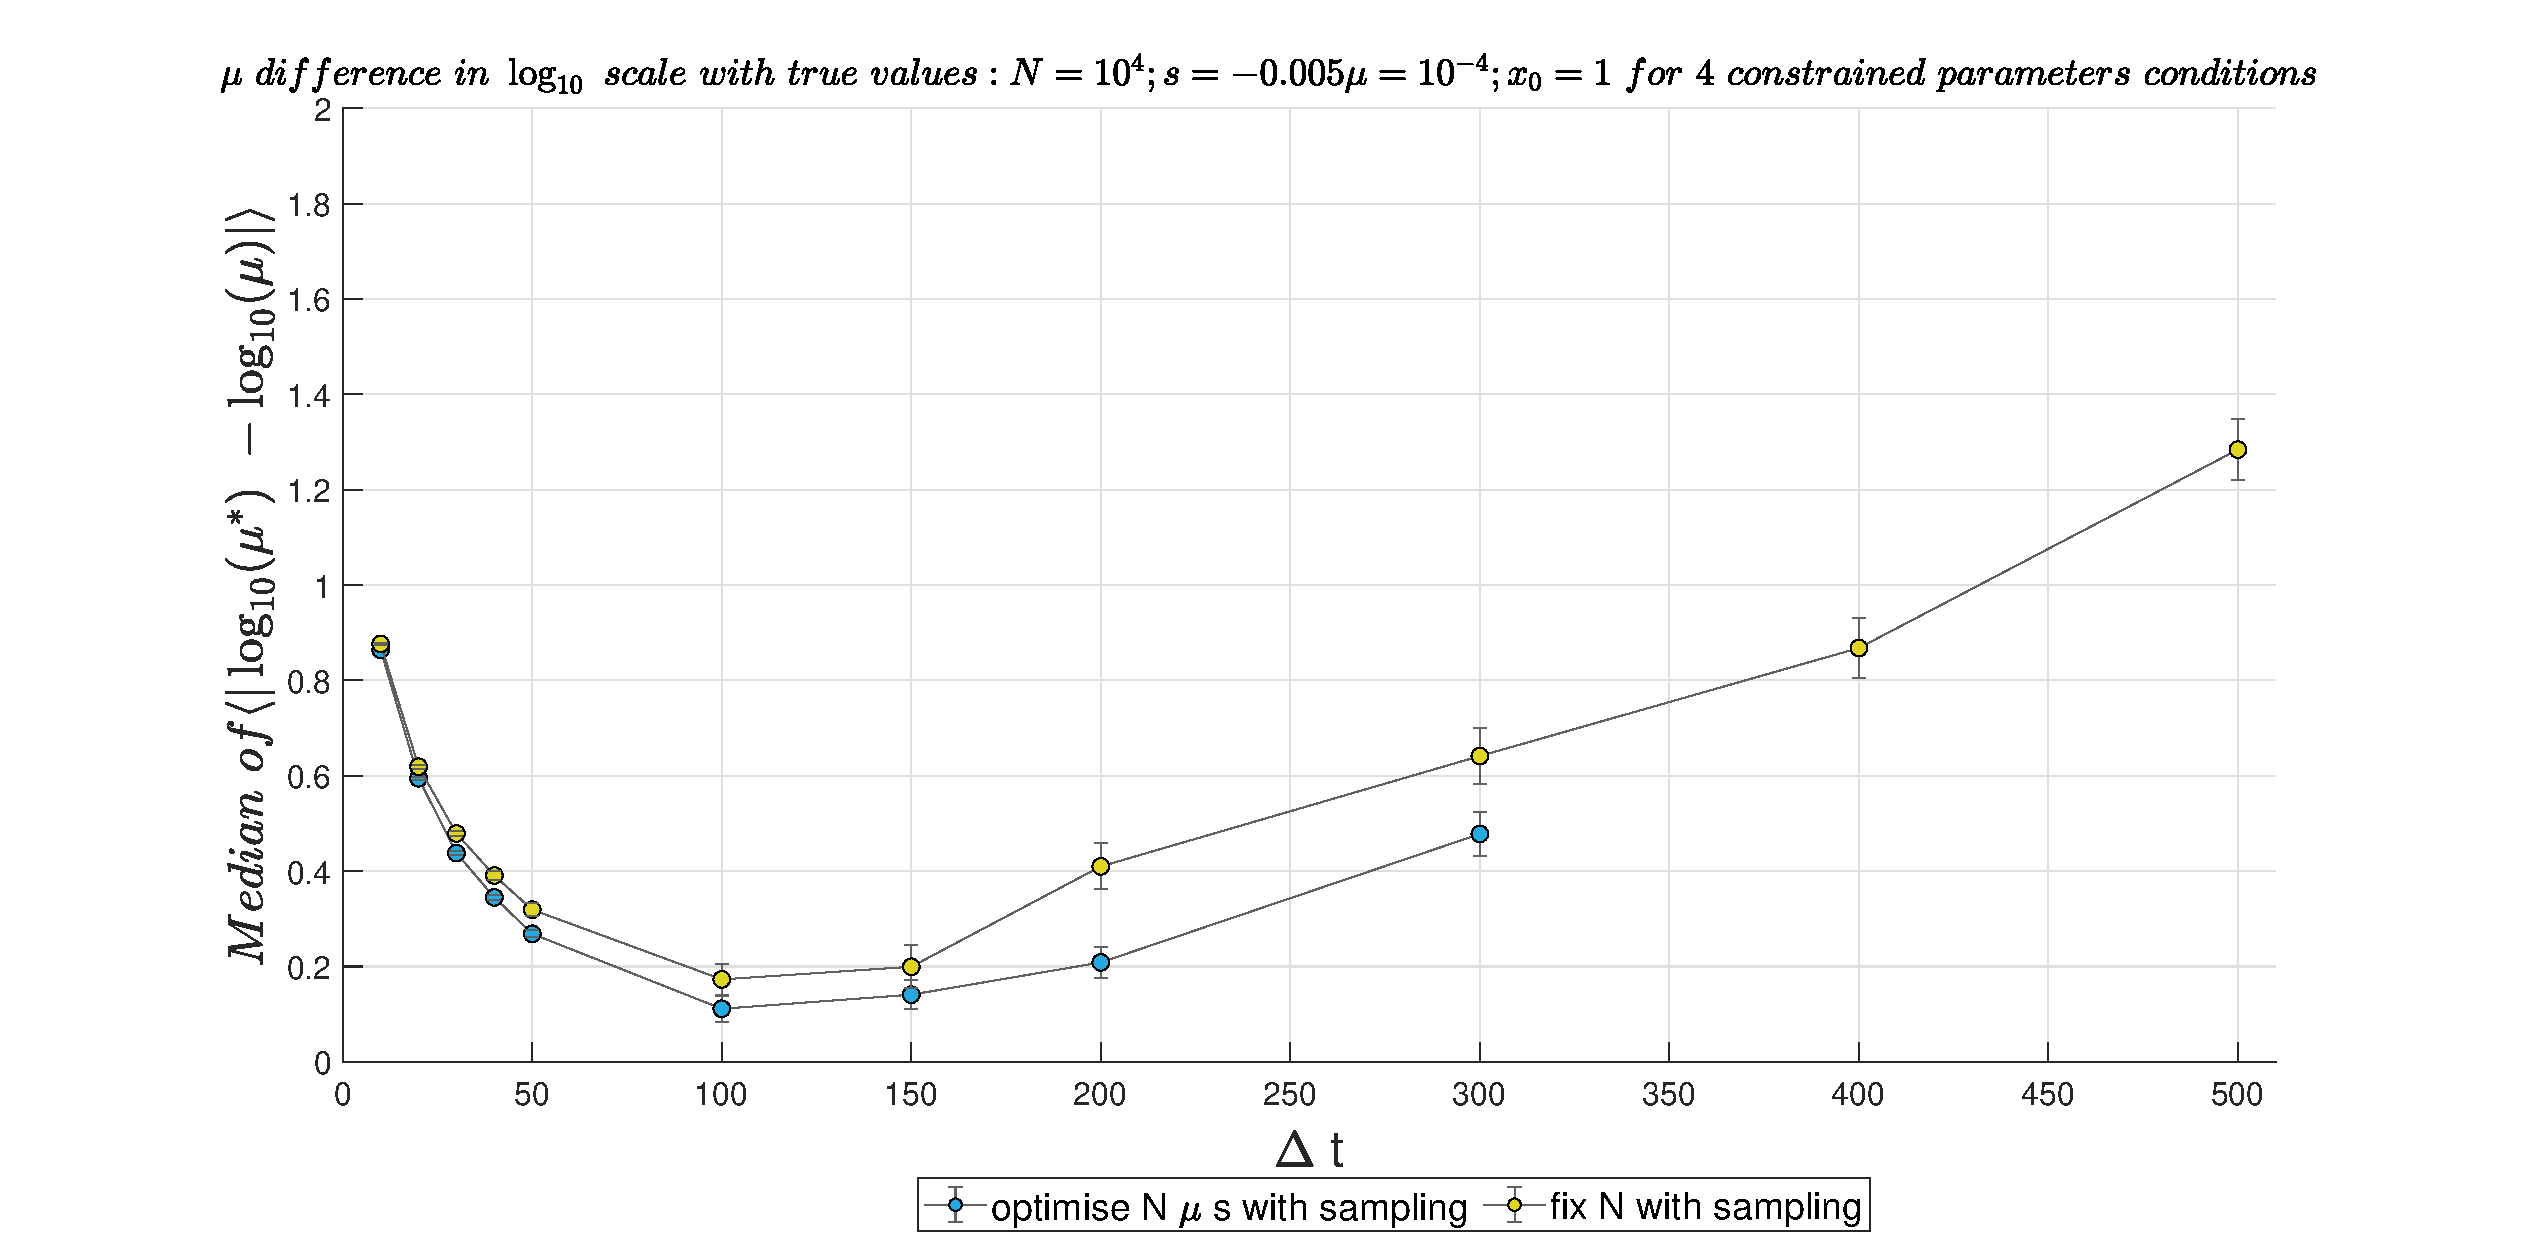
\includegraphics[width=1.6\textwidth,height=0.4\textheight]{figures/mu_neg.eps}}
    \put(10,0){\textcolor{black}{\textbf{C}}}
    \caption{\textbf{$s\ N\ \mu$ error for single site negative selection} A is $s$ error plot, B is $N$ error plot and C is $\mu$ error plot. Different colours indicates different parameters constrained conditions. }

    \label{fig:pt6_pvalue}
\end{figure}
\subsection{Genome-wide simulation and AUC results}
This AUC in this study is to test the performance of the parameter optimisation analysis method in distinguishing whether the site is under selection (ROC plots for each condition can be found in appendix). From the left plot of \textbf{Figure.5}, at $T=1000$, the sampled performance is worse than the non-sampled results. The sampled results are also more volatile. Overall, it seems that fixing the value of $\mu$ and optimising three parameters are most stable under the condition of without sampling and can better distinguish the selection and neutral.
\begin{figure}[H]
    \centering
    \hspace{-1cm}
    \makebox[\textwidth][c]{\includegraphics[width=1.4\textwidth]{figures/AUC_genome-wide.eps}}
    \caption{\textbf{Genome-wide AUC value under different conditions for both positive selection and negative selection sites.} This plot shows AUC value for different T (T=1000 on left, T=10000 on right). Different colours indicates whether fix $N$, $\mu$ parameters conditions. Dash lines are results that simulations are done by binomial sampling, whereas straight lines are not.}
    \label{fig:AUC_value}
\end{figure}
 From the plot on the right, the result of T=10000, results with sampling are even better and stable. Besides, AUCs are mostly maintained at the level of 0.8-0.9. For the unsampled results, the results displayed by AUC at $\Delta t=50$ and $100$ indicate that they cannot distinguish the selection from the neutral situation very well. Fixing $N$, $\mu$ and fixing $\mu$ with sampling are optimal among all conditions when T=10000. In view of the overall situation, the sampling with fixed $N\ \mu$ value performed the best. Although when $\Delta t=5,20$, AUC are low at these conditions, but compared with other conditions at the same other sampling time, it has more higher AUC.\\

 Obtaining the ROC curve (\textbf{Figure. 6}) of the case with the highest AUC, which is $T=10000, \Delta t=100 with sampling$, can see the specific situation of classifying selection and neutrality of sites. The optimal threshold selection can control the FPR less than 0.1 and the TPR slightly higher than 0.7.

 \begin{figure}[H]
    \centering
    \hspace{-1cm}
    \makebox[\textwidth][c]{\includegraphics[width=1.4\textwidth]{figures/ROC_T10000_dt100.eps}}
    \caption{\textbf{ROC for T=10000 dt=100.} This plot shows ROC for $T=10000, \Delta t=100$ in fixing $N\ \mu$ condition. The AUC in this condition is the highest among AUC value shows in previous figure.}
    \label{fig:AUC_value}
\end{figure}



\subsection{SARS-CoV-2 Patient analysis results}
Apply analysis method proposed by \cite{khatri2016quantifying} based on WF model to the data of two groups of immunocompromised patients infected by SARS-CoV-2 virus, the following results can be obtained. First, \textbf{Figure. 7 (A,B)} are the histograms of the $p-values$ in different fixing parameter cases for both patient 6 and 9. The the $p-values$ increase sequentially from left to right. The red dash lines in the figures indicate the threshold value of the adjusted $p-value$ obtained by the BH method, and all $p-values$ smaller than the dash lines are significant, and vice versa. Max count indicates the frequency of the highest bin. Ideally, p should be peaked towards 0 and tail off to a constant close to 1. From the \textbf{(Figure.7(A))}, for patient 6, it can be clearly seen that when the three sets of parameters are optimised, the proportion of the left part of the threshold is very low. When it turns to fixing $N$, fixing $\mu$ and fixing $N\ \mu$, the results are much better then the first condition, more than 18000 locus are significant under selection.  This means that detecting selection with optimising $N\ \mu\ s$ might be problematic in the case of patient 6. From the \textbf{(Figure.7(B))}, for patient 9, expect optimising $N\ \mu\ s$ has a low significant sites results, fixing $\mu$ in this case becomes worse then it in patient 6 case. Overall, regardless of the parameters constrained situations, it seems that once $N$ is fixed the multi-hypothesis results would get better, more sites are significant.\\

From the perspective of the distribution of the entire $p-value$, the performance of simultaneously optimising three sets of parameters is very unsatisfactory, because it has a peak at a position where the $p-value$ is close to 1. The distributions of the other three groups are relatively good.\\
\begin{figure}[H]
    \centering
    \hspace{-1cm}
    \makebox[\textwidth][c]{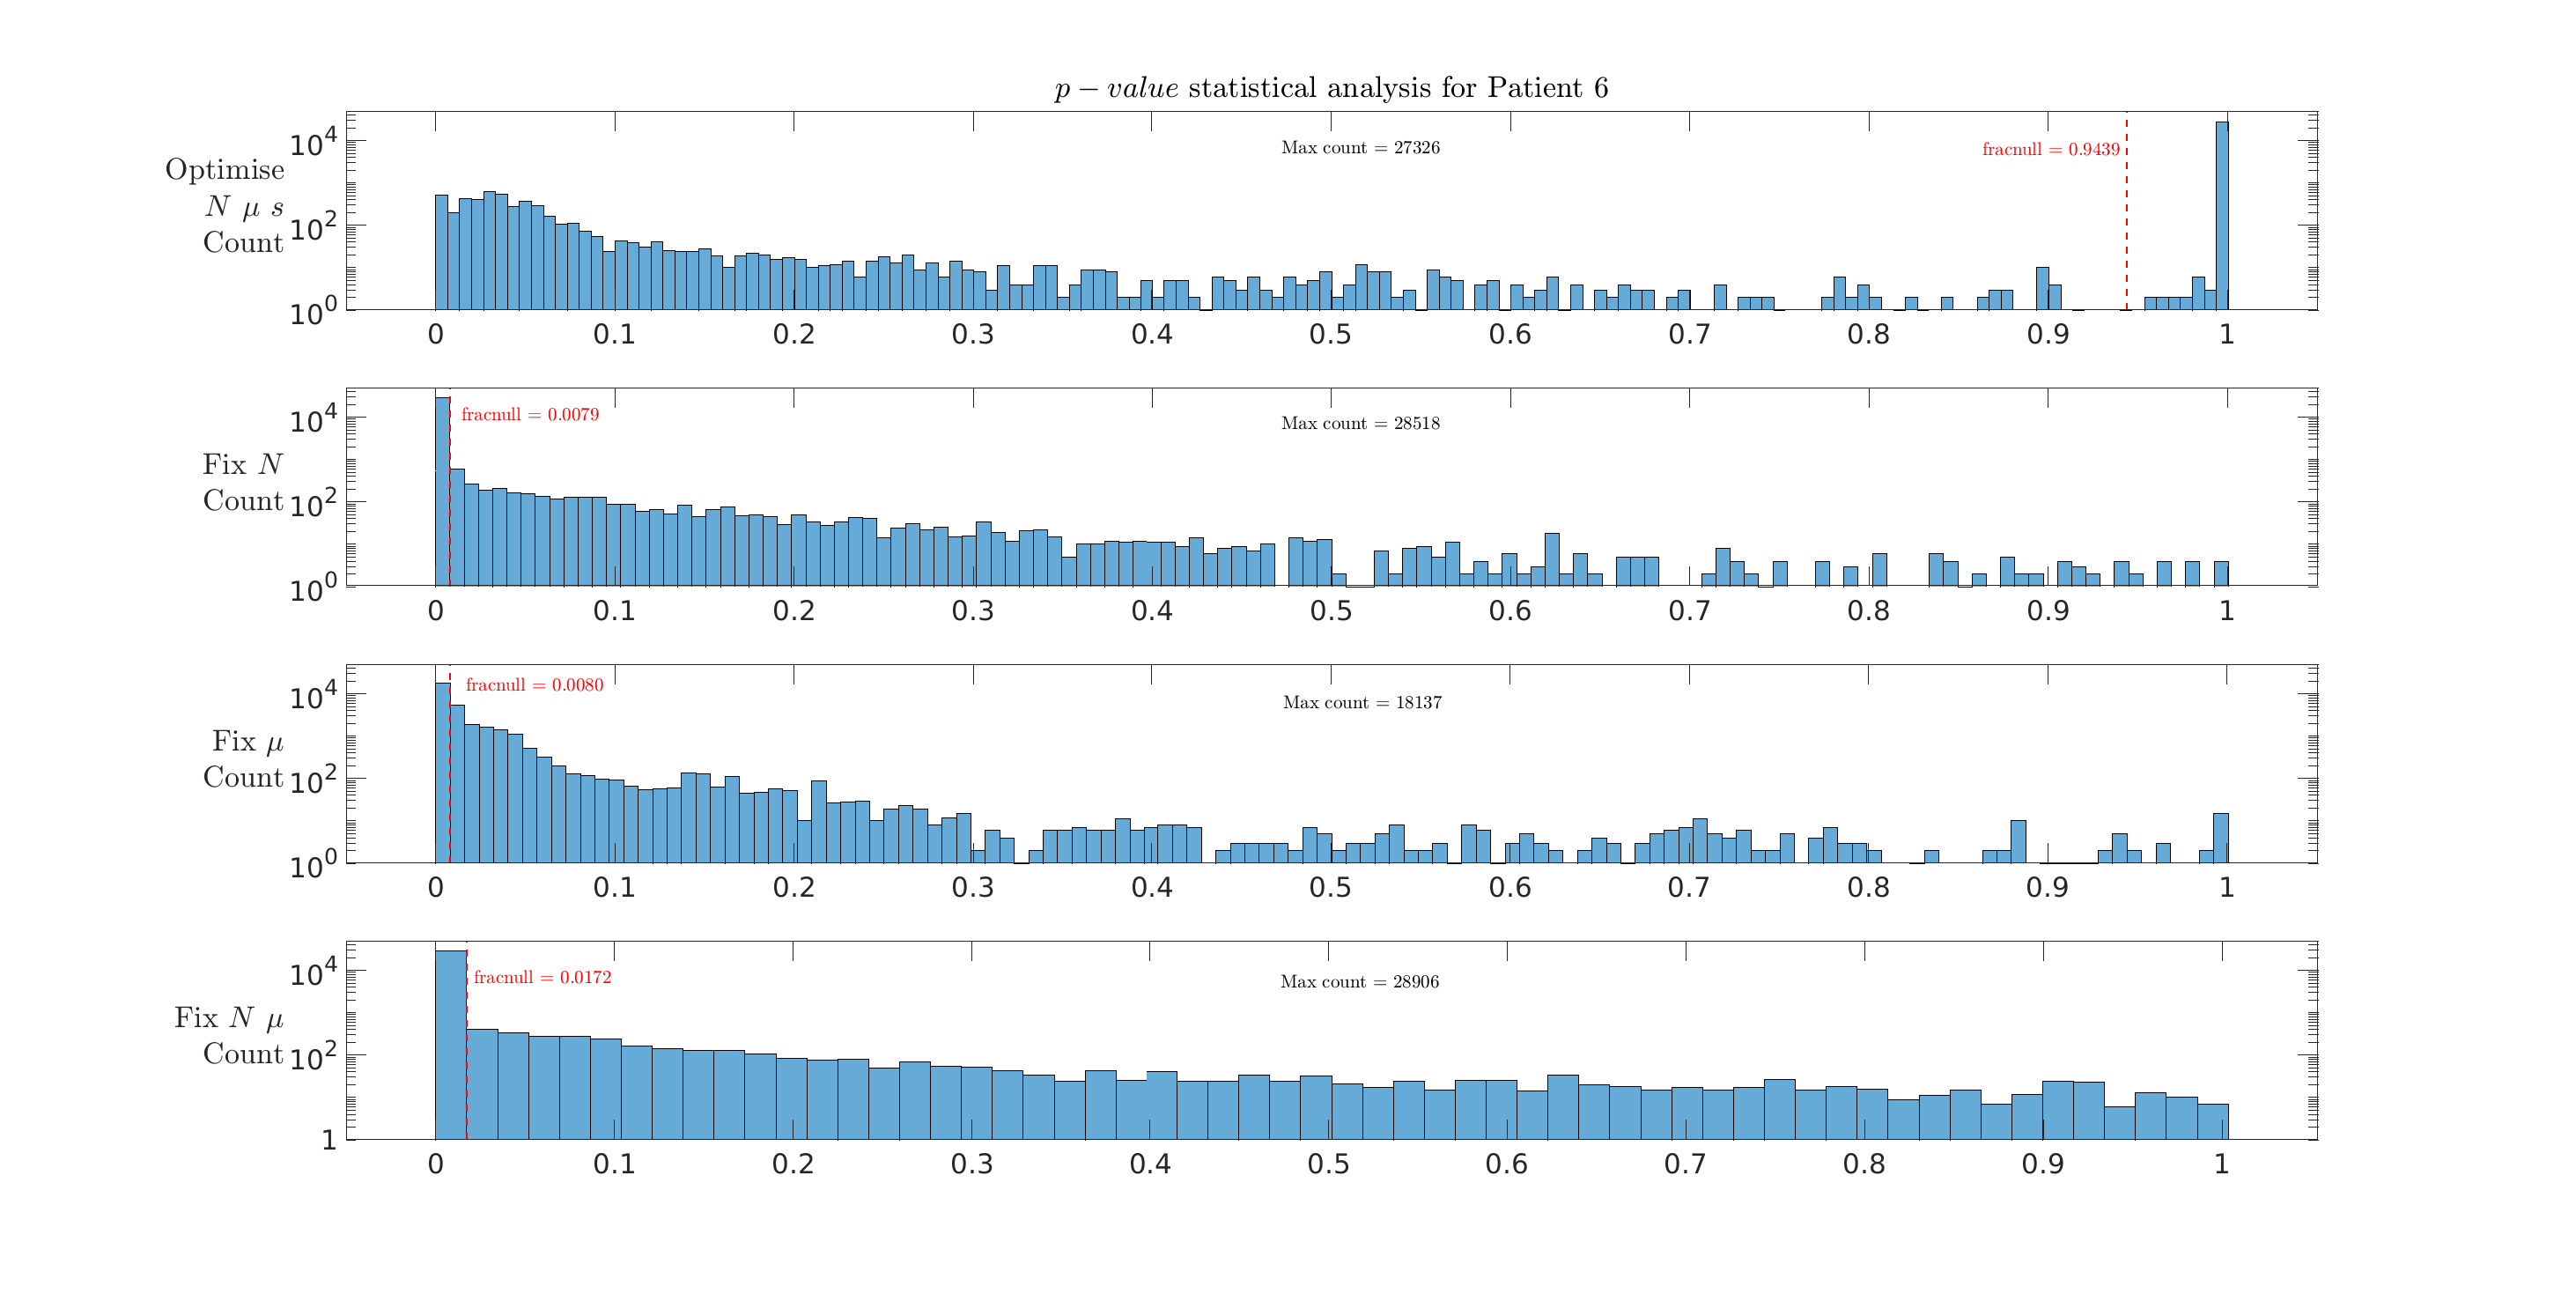
\includegraphics[width=1.6\textwidth,height=0.4\textheight]{figures/patient/pt6/pt6_pvalue.eps}}
    \put(0,0){\textcolor{black}{\textbf{A}}}
    \label{fig:pt6_pvalue}
\end{figure}

\begin{figure}[H]
    \centering
    \hspace{-1cm}
    \makebox[\textwidth][c]{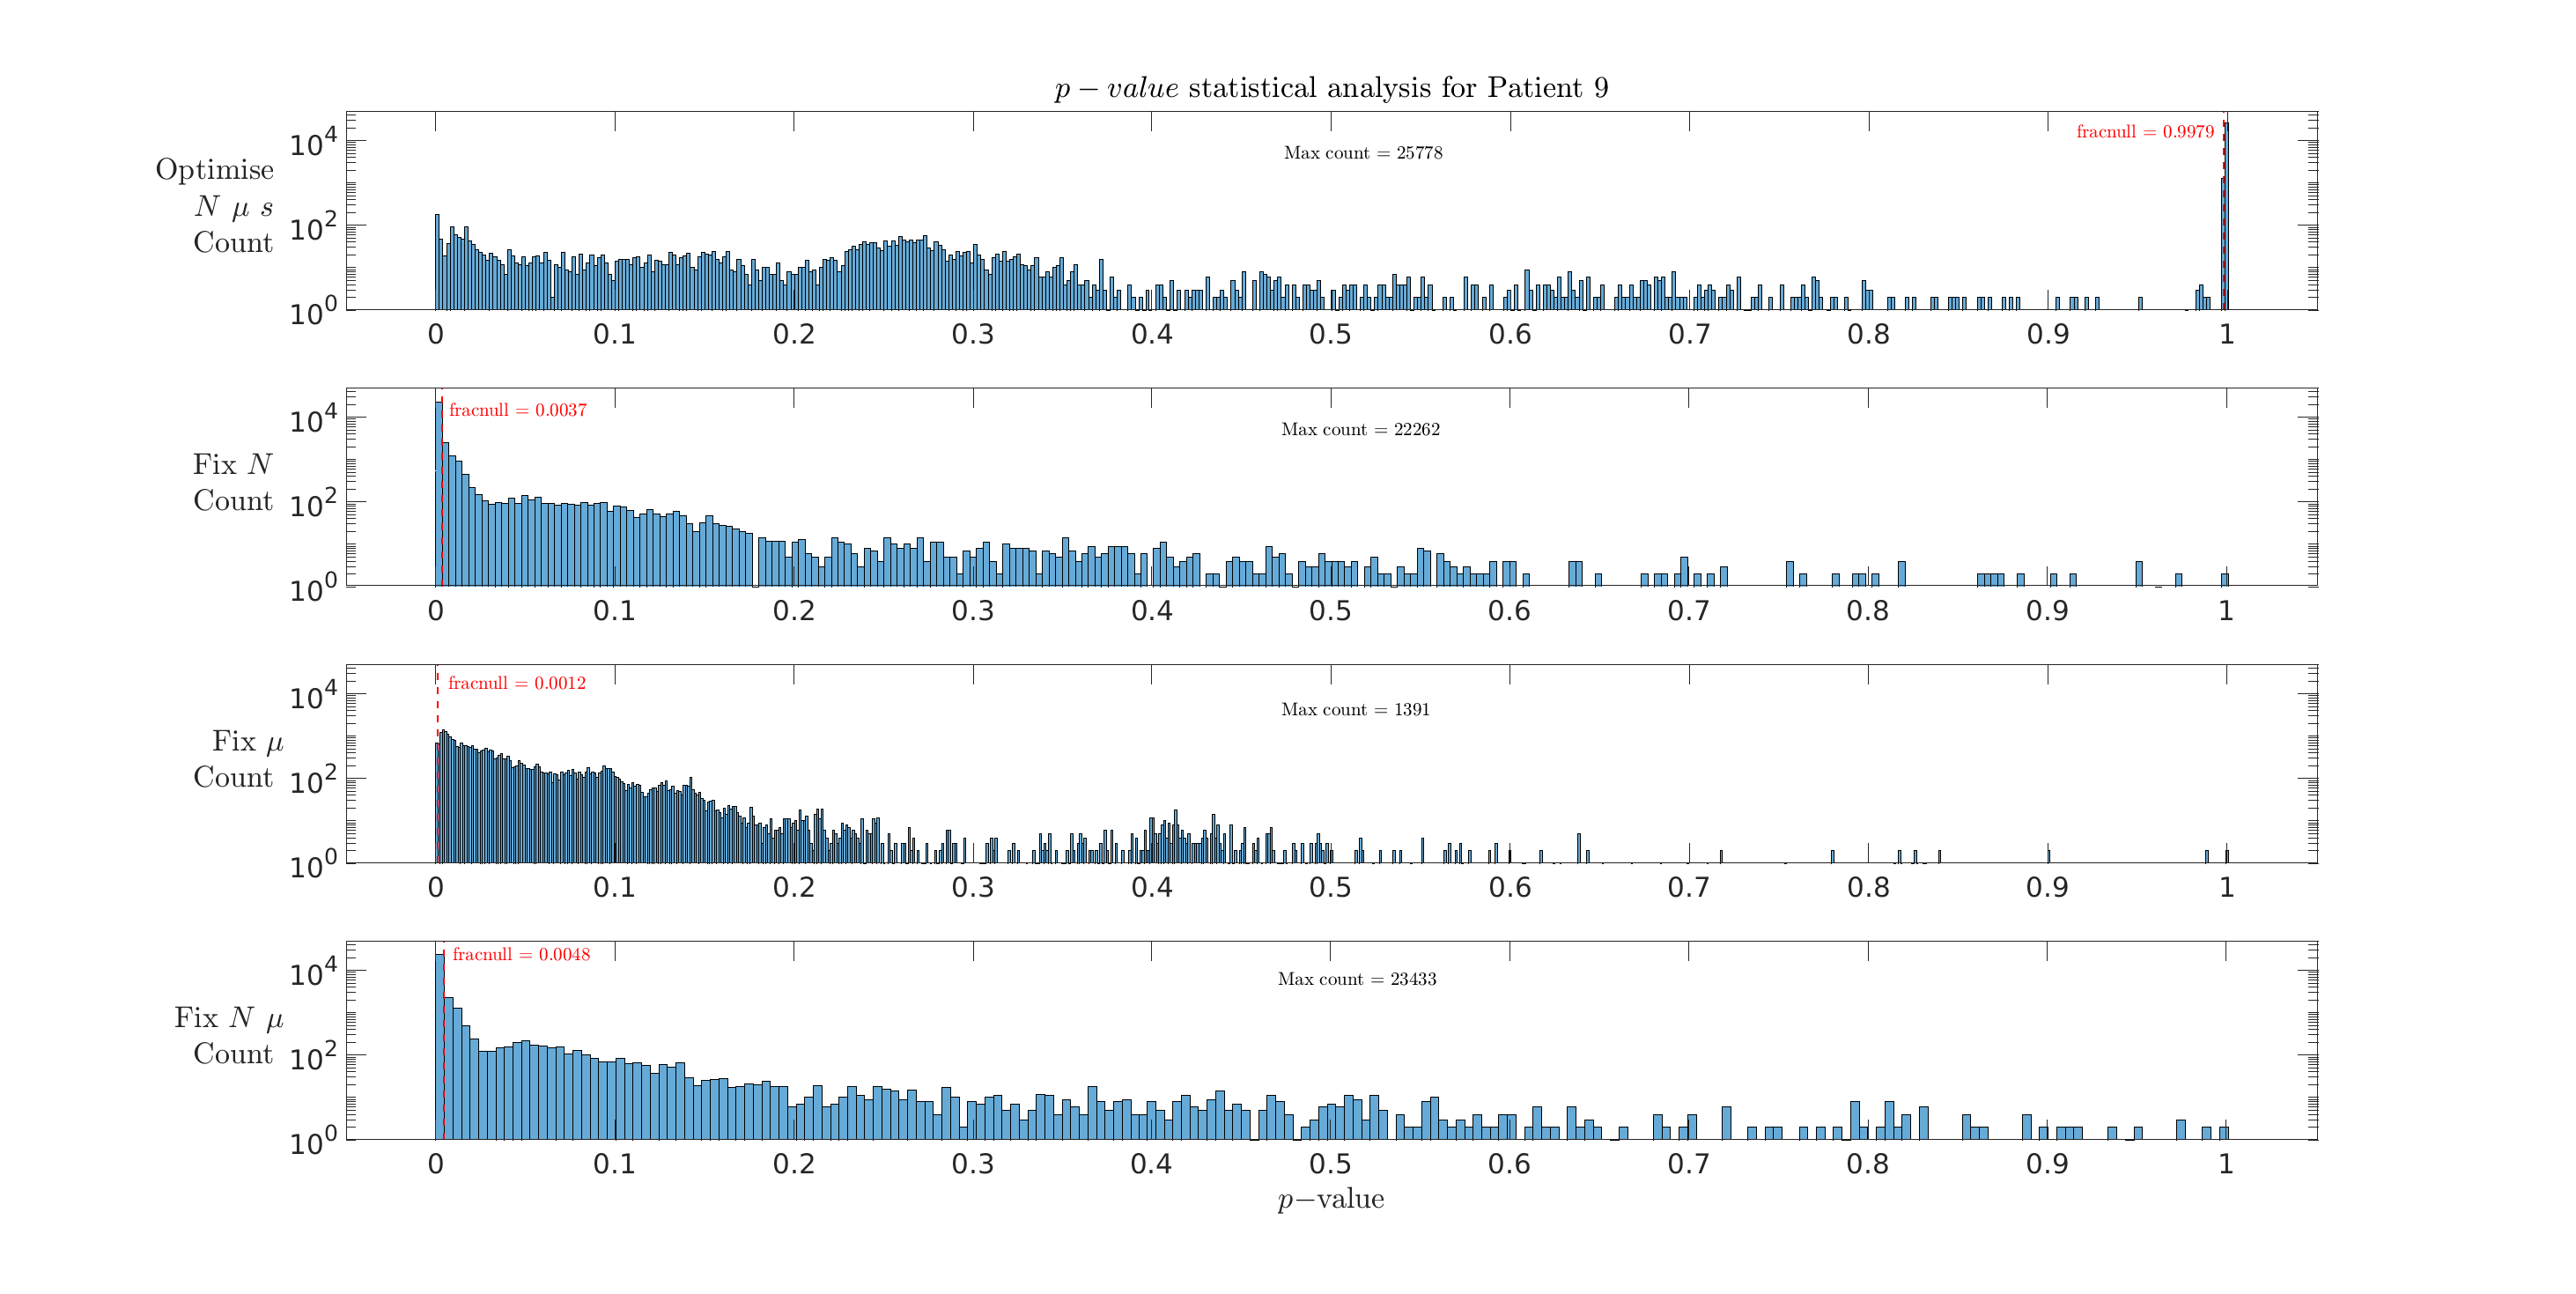
\includegraphics[width=1.6\textwidth,height=0.4\textheight]{figures/patient/pt9/pt9_pvalue_all.eps}}
    \put(0,0){\textcolor{black}{\textbf{B}}}
    \caption{\textbf{p-value histogram for patient 6 (A) and 9 (B) under 4 different cases.} This figure is a frequency histogram of $p-value$. Four subplots represent four cases where the parameters are fixed. The red dash line indicates the threshold of the null hypothesis. If it is less than this value, it means that the p-value is significant.}
    \label{fig:pt9_pvalue}
\end{figure}

\textbf{Figure 8} and \textbf{Figure 9} show the DFE of optimised s in 4 parameters constrained situations. We mentioned in the previous part that most of sites in gene are neutral selection, so $s$ is very small. And the distribution of $s$ satisfies the exponential distribution. In the results of \textbf{Figures 8 and 9}, it can be seen that among the results of four parameter optimisation choices, the DFE distribution under fixed N \textbf{Figures 8(b)} and fixing $N\ \mu$ \textbf{Figures 9(d)} is closest to an exponential distribution from zero to negative (because in most sites s<0, the closer selection coefficient to zero, the closer to neutral). Therefore, the result basically satisfies the above-mentioned point of view, and the detection on the selected sites is better under fixing $N$ and fixing $N$ $\mu$.\\

\begin{figure}[H]
    \centering
    
    \begin{subfigure}{1\textwidth}
        \includegraphics[width=\linewidth]{figures/patient/pt6/pt6_DFE_s.eps}
        \caption{DFE for optimising $N\ \mu\ s$ for patient 6}
        \label{fig:subfig1}
    \end{subfigure}
    
    \begin{subfigure}{1\textwidth}
        \includegraphics[width=\linewidth]{figures/patient/pt6/pt6_fixN_DFE_s.eps}
        \caption{DFE for fixing $N$ for patient 6}
        \label{fig:subfig2}
    \end{subfigure}
     \end{figure}

\begin{figure}[H]
    \ContinuedFloat
   
    
    \begin{subfigure}{1\textwidth}
        \includegraphics[width=\linewidth]{figures/patient/pt6/pt6_fixmu_DFE_s.eps}
        \caption{DFE for fixing $\mu$ for patient 6}
        \label{fig:subfig3}
    \end{subfigure}
    \hfill
    \begin{subfigure}{1\textwidth}
        \includegraphics[width=\linewidth]{figures/patient/pt6/pt6_fixNmu_DFE_s.eps}
        \caption{DFE for fixinging $N\ \mu$ for patient 6}
        \label{fig:subfig4}
    \end{subfigure}
    
    \caption{\textbf{DFE in 4 parameters constrained situation for patient 6} This group of graphs shows the probability density distribution (pdf) of the optimised selection coefficient of patient 6, that is, the fitness effect distribution. For details, please refer to the method section.}
    \label{fig:four_subfigs}
\end{figure}

\begin{figure}[H]
    \centering
    
    \begin{subfigure}{1\textwidth}
        \includegraphics[width=\linewidth]{figures/patient/pt6/pt6_DFE_s.eps}
        \caption{DFE for optimising $N\ \mu\ s$ for patient 9}
        \label{fig:subfig1}
    \end{subfigure}
    
    \begin{subfigure}{1\textwidth}
        \includegraphics[width=\linewidth]{figures/patient/pt9/pt9_fixN_DFE_s.eps}
        \caption{DFE for fixing $N$ for patient 9}
        \label{fig:subfig2}
    \end{subfigure}
    
     \end{figure}

\begin{figure}[H]
    \ContinuedFloat
    
    \begin{subfigure}{1\textwidth}
        \includegraphics[width=\linewidth]{figures/patient/pt9/fixmu_DFE_s.eps}
        \caption{DFE for optimising $\mu$ for patient 9}
        \label{fig:subfig3}
    \end{subfigure}
    \hfill
    \begin{subfigure}{1\textwidth}
        \includegraphics[width=\linewidth]{figures/patient/pt9/pt9_fixNmu_DFE_s.eps}
        \caption{DFE for optimising $N\ \mu$ for patient 9}
        \label{fig:subfig4}
    \end{subfigure}
    
    \caption{\textbf{DFE in 4 parameters constrained situation for patient 9} This group of graphs shows the probability density distribution (pdf) of the optimised selection coefficient of patient 9, that is, the fitness effect distribution.}
    \label{fig:four_subfigs}
\end{figure}

\textbf{Figure 10} and \textbf{Figure 11} show the selected sites within SARS-CoV-2 virus under 4 parameters constrained situations. According to the above situation, since the results of fixing $N$ and fixing $N$ $\mu$ are more reliable, we can find the corresponding selection sites lollipop plots(\textbf{Figure 10} and \textbf{Figure 11}) of the two cases for verifying. It can be found that whether it is patient 6 or 9, the selected sites among positive selection sites in these two cases are also closer. Compared with the above-mentioned cases, the positive selected sites of the other two limited parameters conditions have some shortcomings. In the case of optimising the three parameters at the same time, it seems that the selected sites cannot be well picked out, and from the results of fixing $\mu$, it seems that all sites' $-log_{10}(q)$ values are significantly higher than $-log_{10}(0.05)$ , it seems that under these two constrained cases, the result is either too strict or too loose.\\



\begin{figure}[H]
    \centering
    \hspace{-6cm}
    \vspace{-4cm}
    \begin{subfigure}{0.7\textwidth}
    \hspace{-2.5cm}
            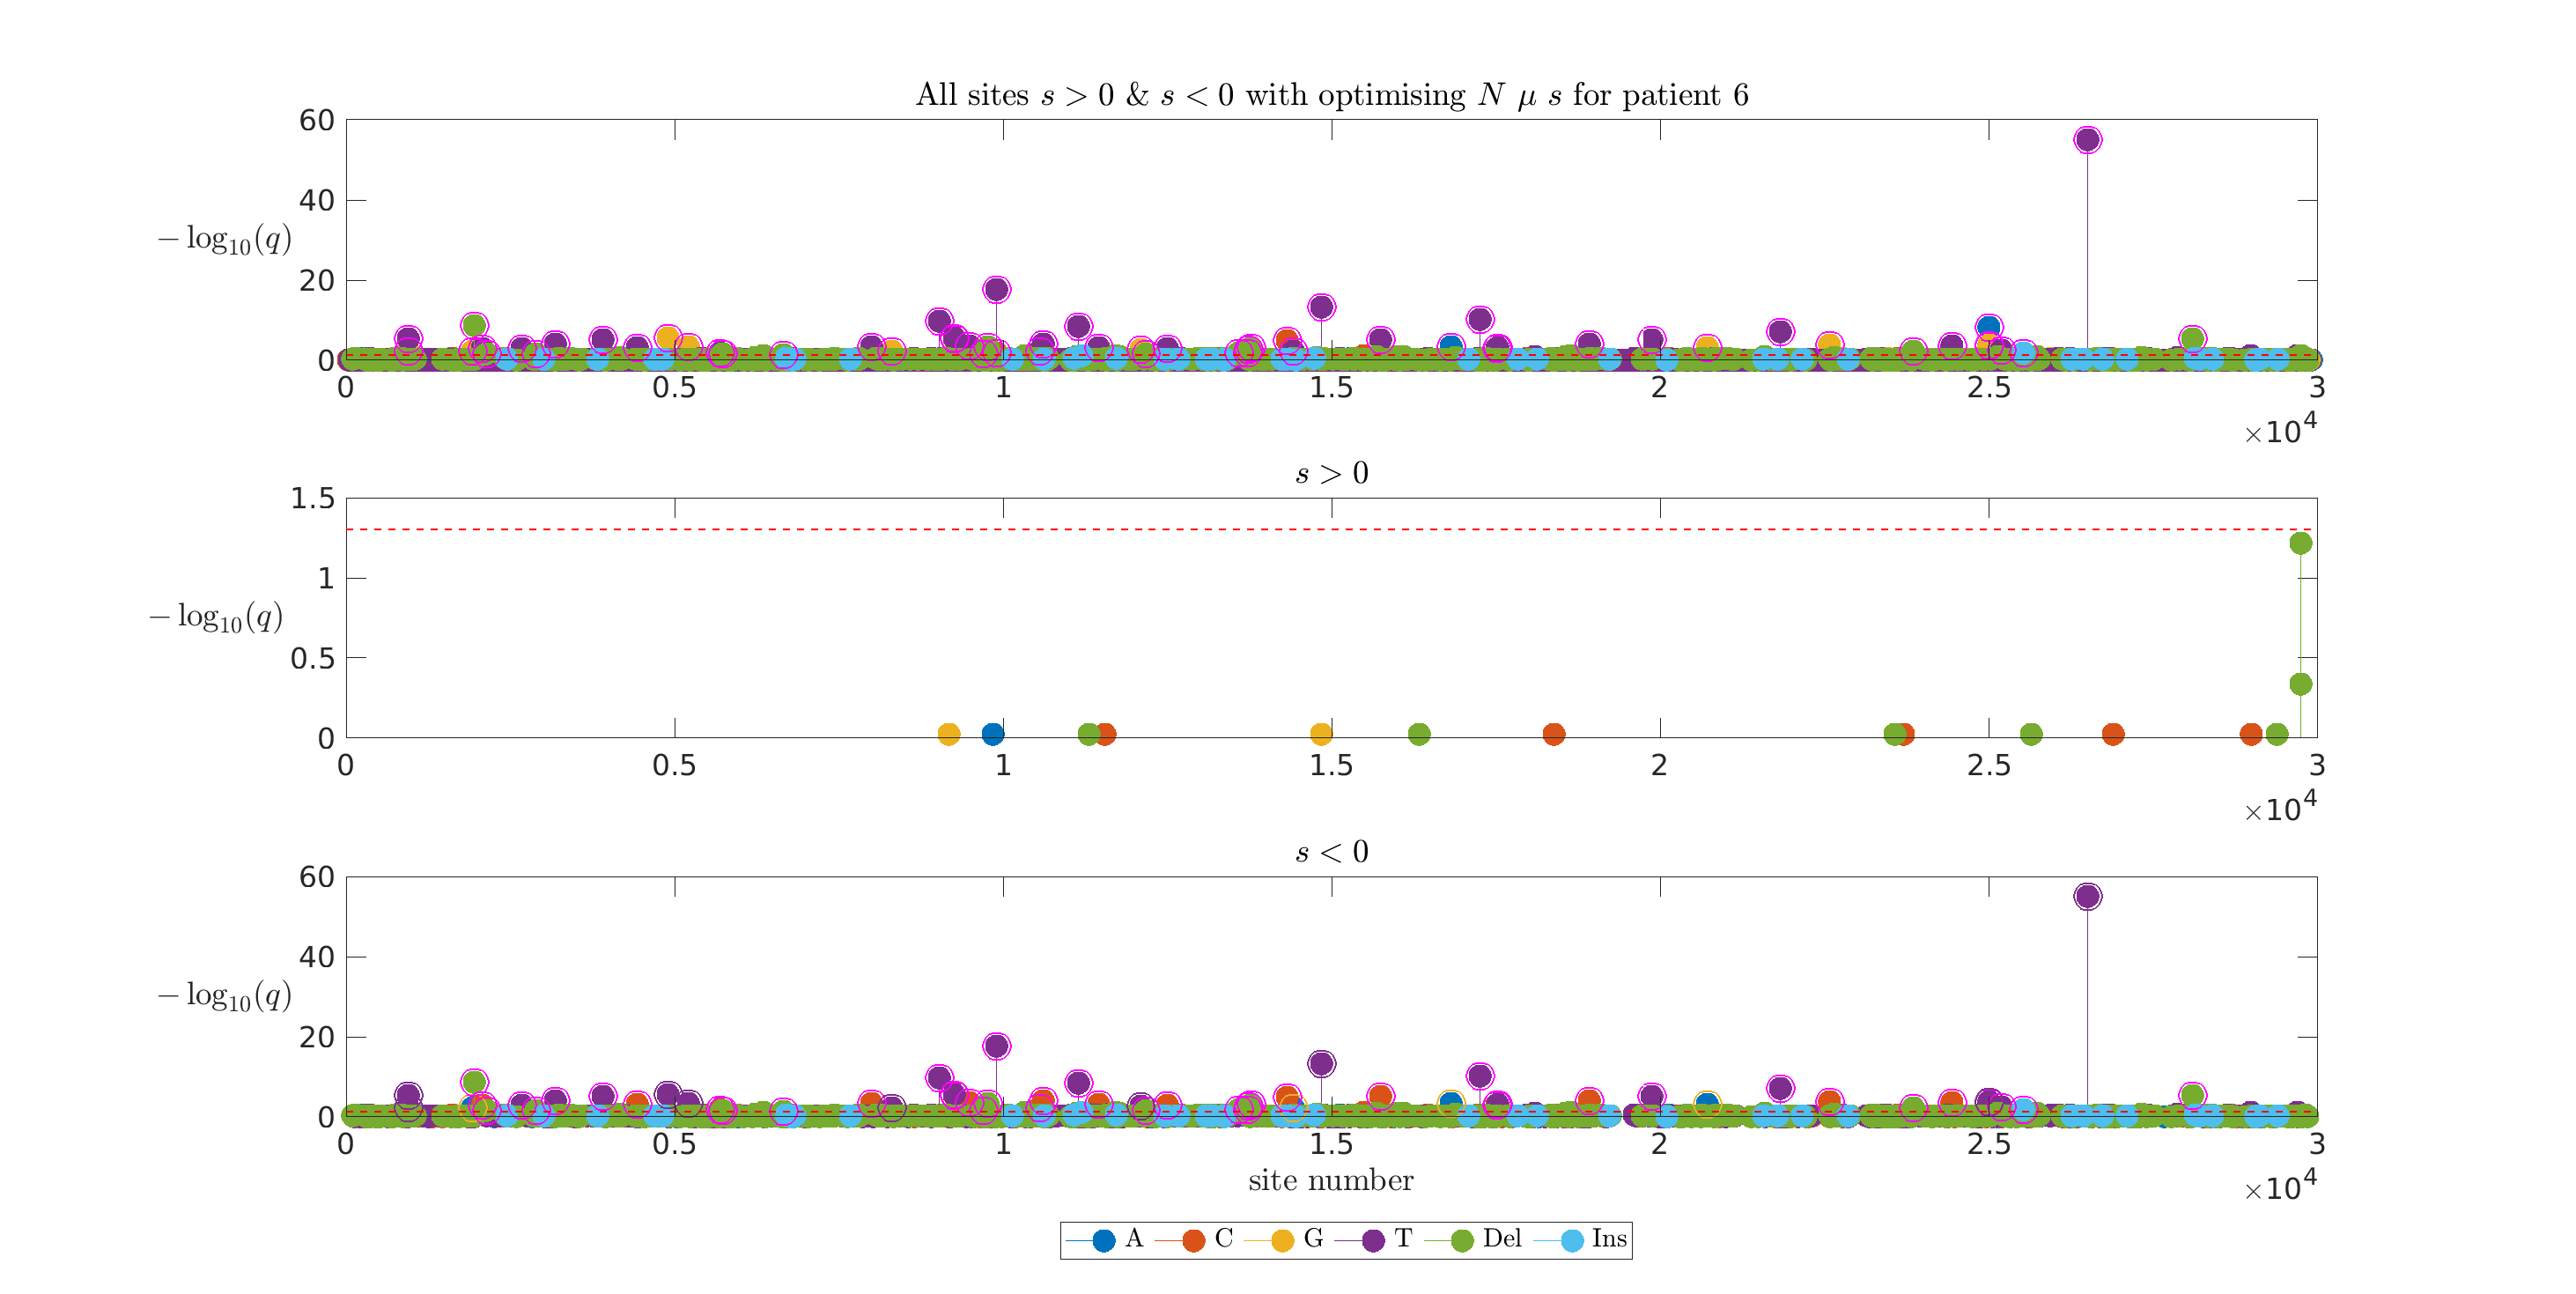
\includegraphics[height=0.5\textheight]{figures/patient/pt6/pt6_site_all_opt.eps}
        
        \caption{Selected site for optimising $N\ \mu\ s$ in patient 6}
        \label{fig:subfig1}
    \end{subfigure}
        \end{figure}

\begin{figure}[H]
    \ContinuedFloat
    \begin{subfigure}{0.7\textwidth}
    \hspace{-2.5cm}
            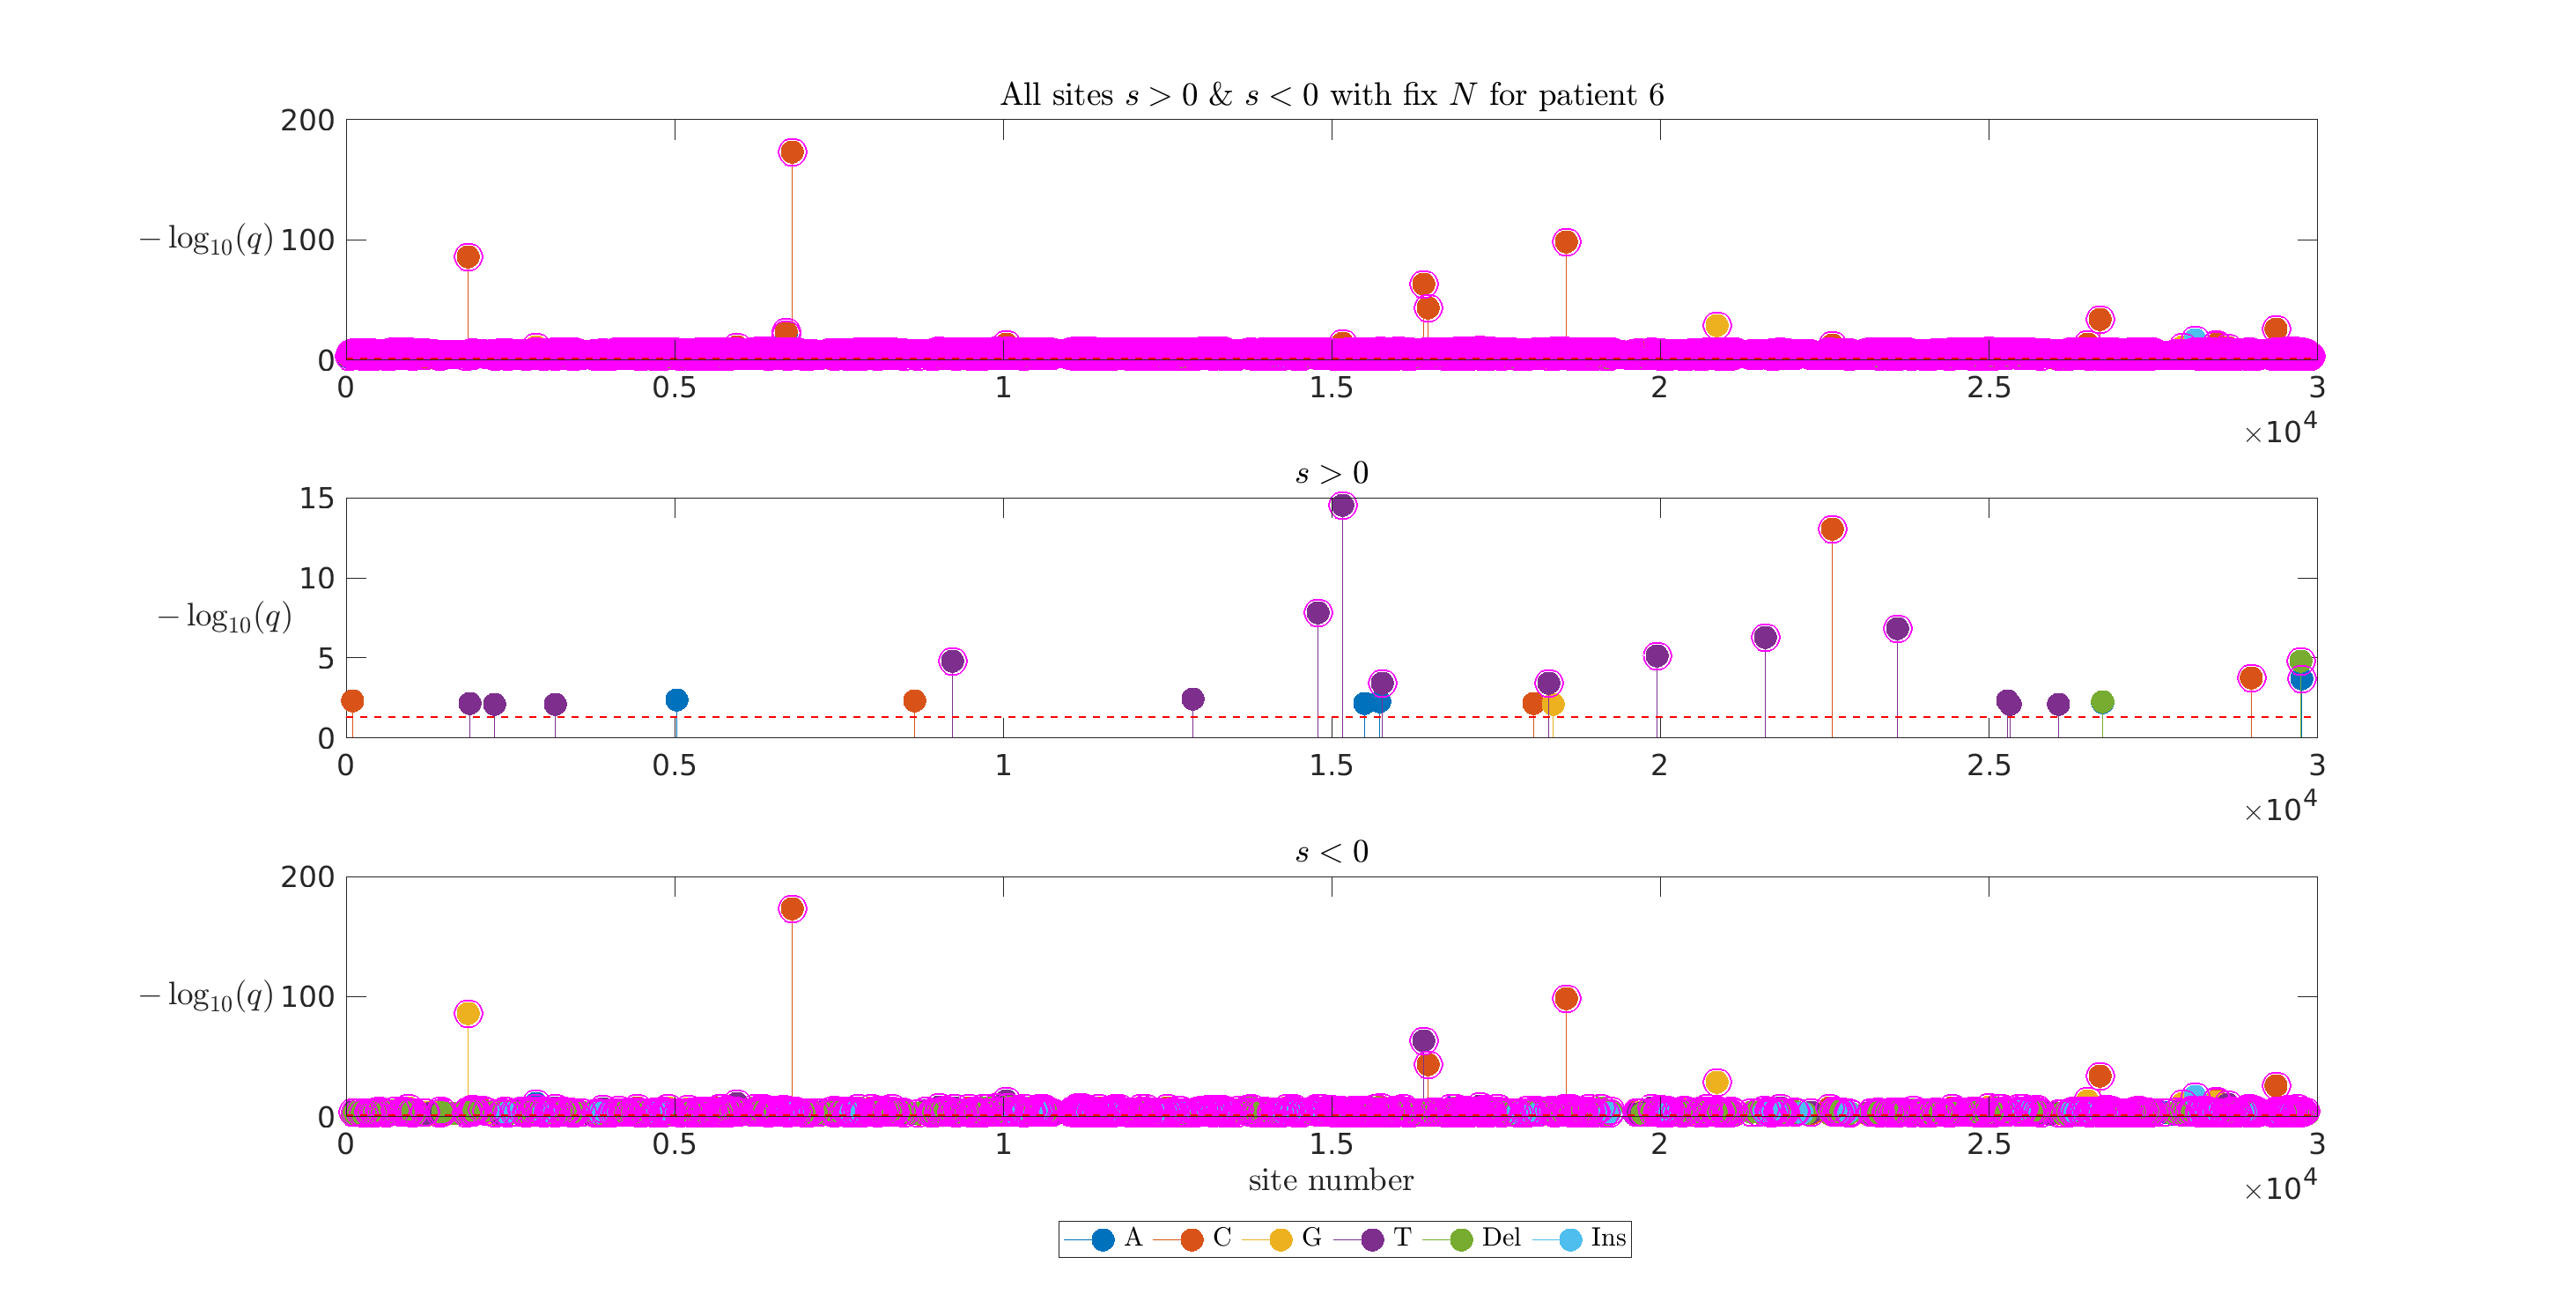
\includegraphics[height=0.5\textheight]{figures/patient/pt6/pt6_siteunder_selection_all_fixN.eps}
       
        \caption{Selected site for fixing $N$ in patient 6}
        \label{fig:subfig2}
    \end{subfigure}
    \end{figure}

\begin{figure}[H]
    \ContinuedFloat
    \vspace{1em} 
    
    \begin{subfigure}{0.7\textwidth}
    \hspace{-2.5cm}
            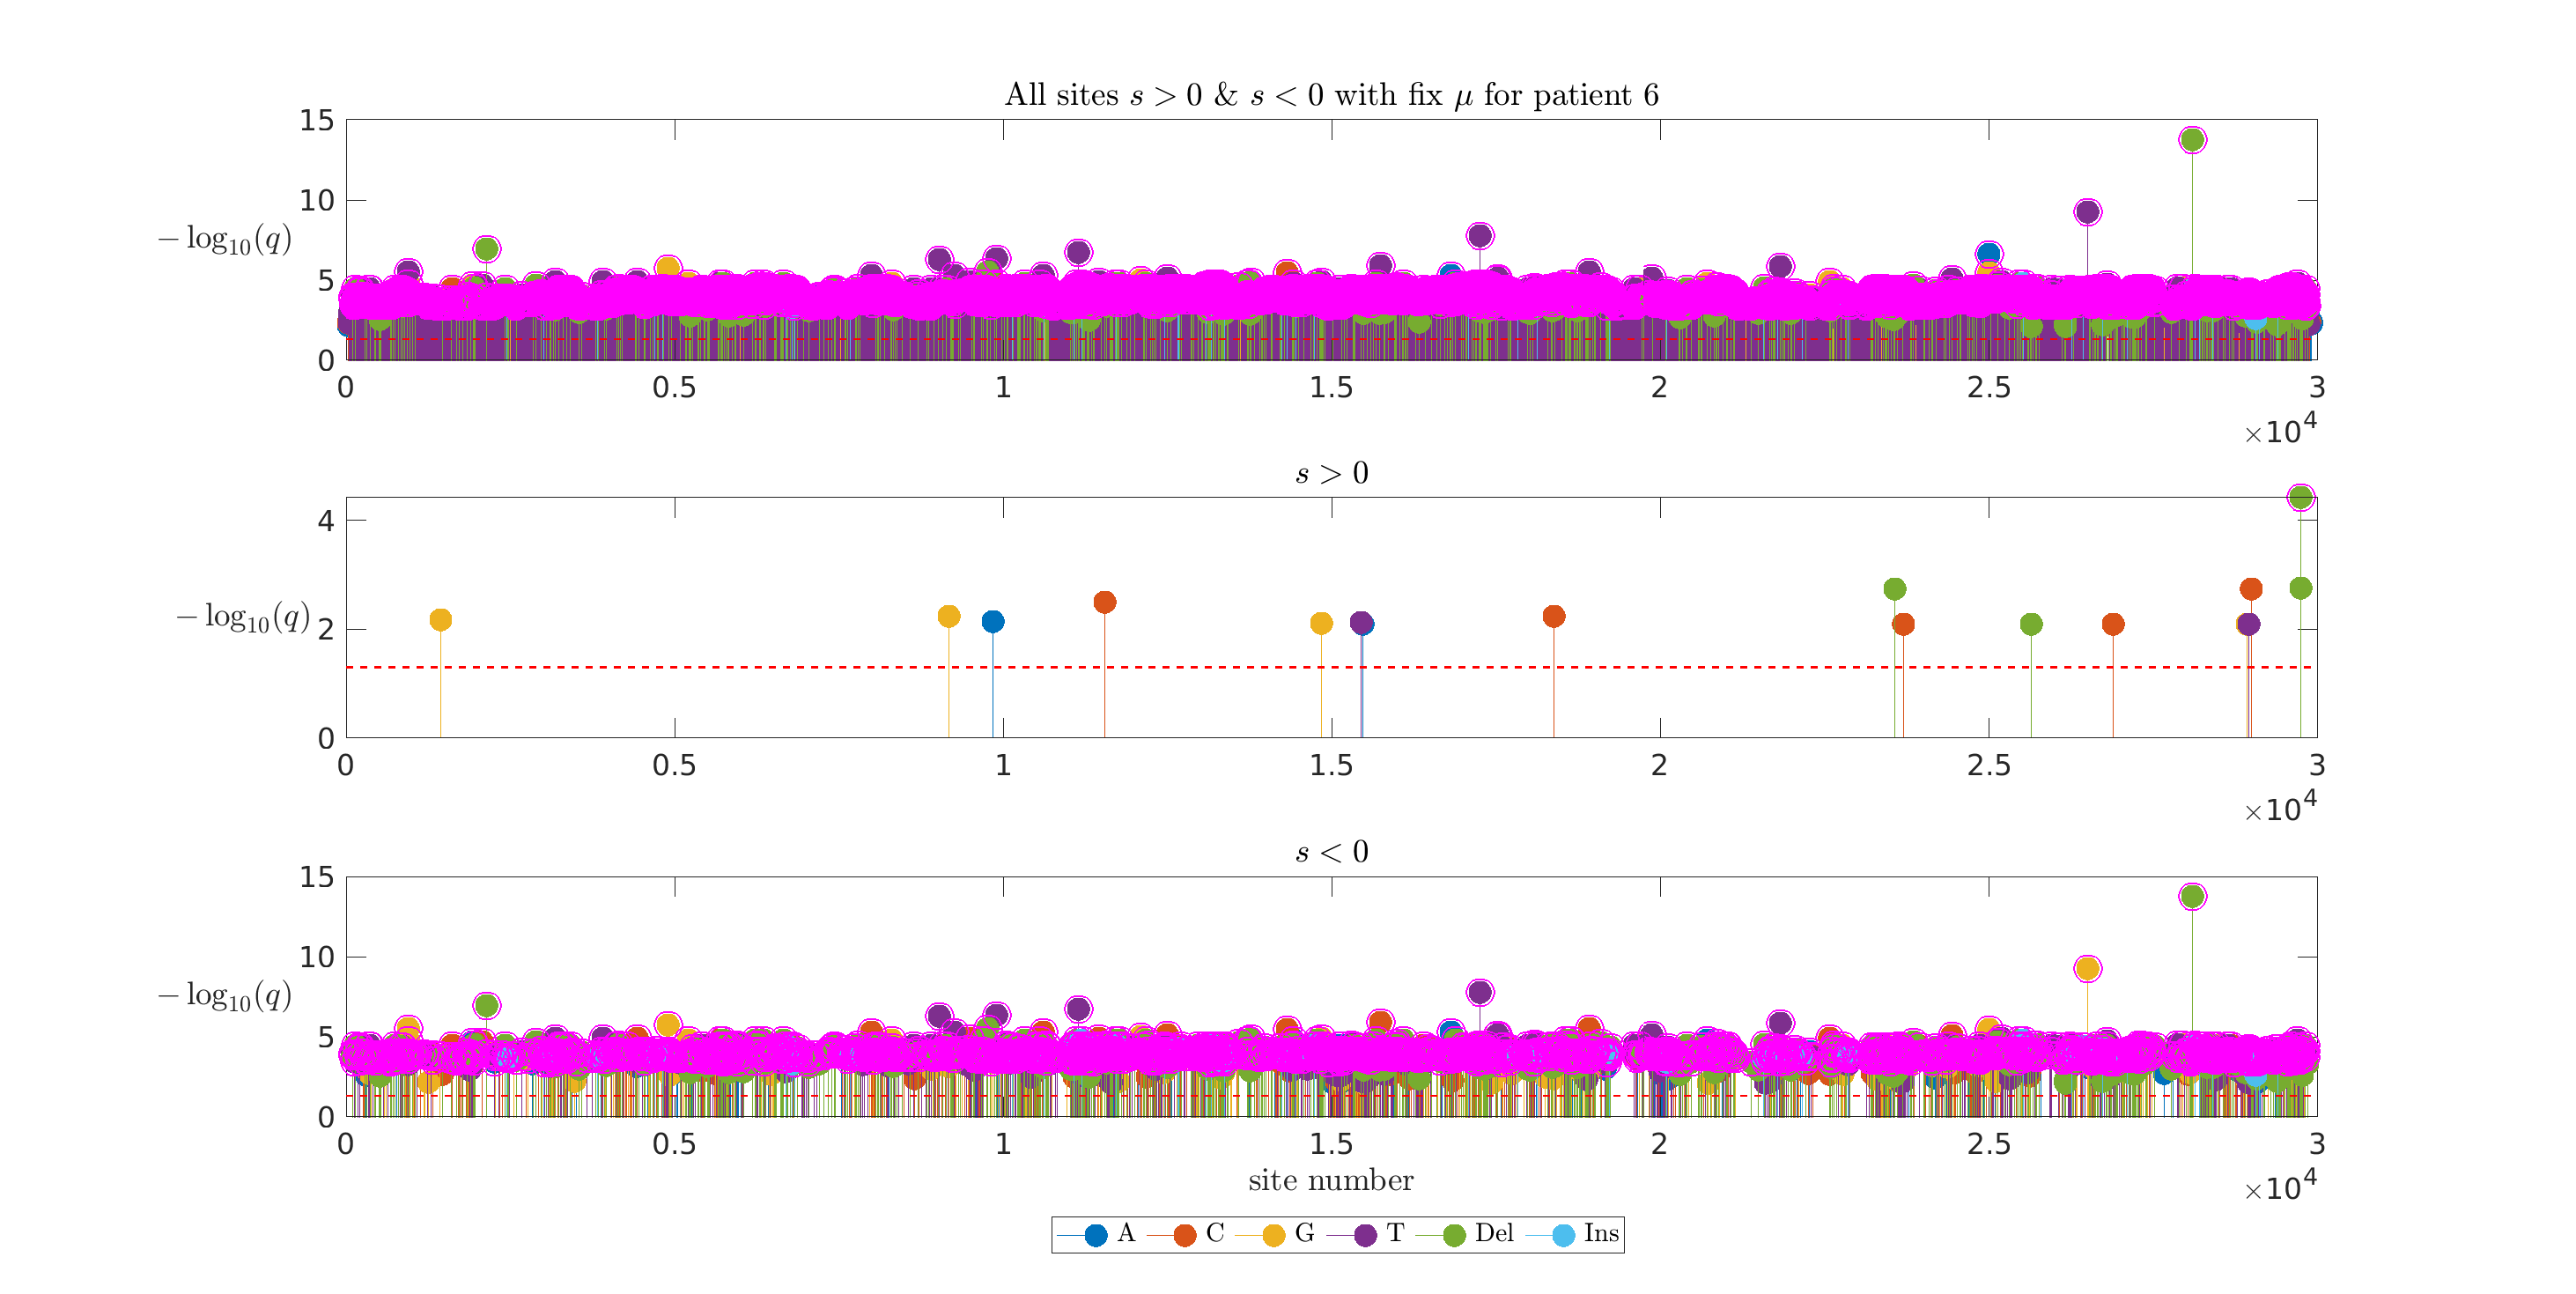
\includegraphics[height=0.5\textheight]{figures/patient/pt6/pt6_siteunder_selection_all_fixmu.eps}
        
        \caption{Selected site for fixing $\mu$ in patient 6}
        \label{fig:subfig3}
    \end{subfigure}
        \end{figure}

\begin{figure}[H]
    \ContinuedFloat

    
    \begin{subfigure}{0.7\textwidth}
    
    
        \hspace{-2.5cm}
            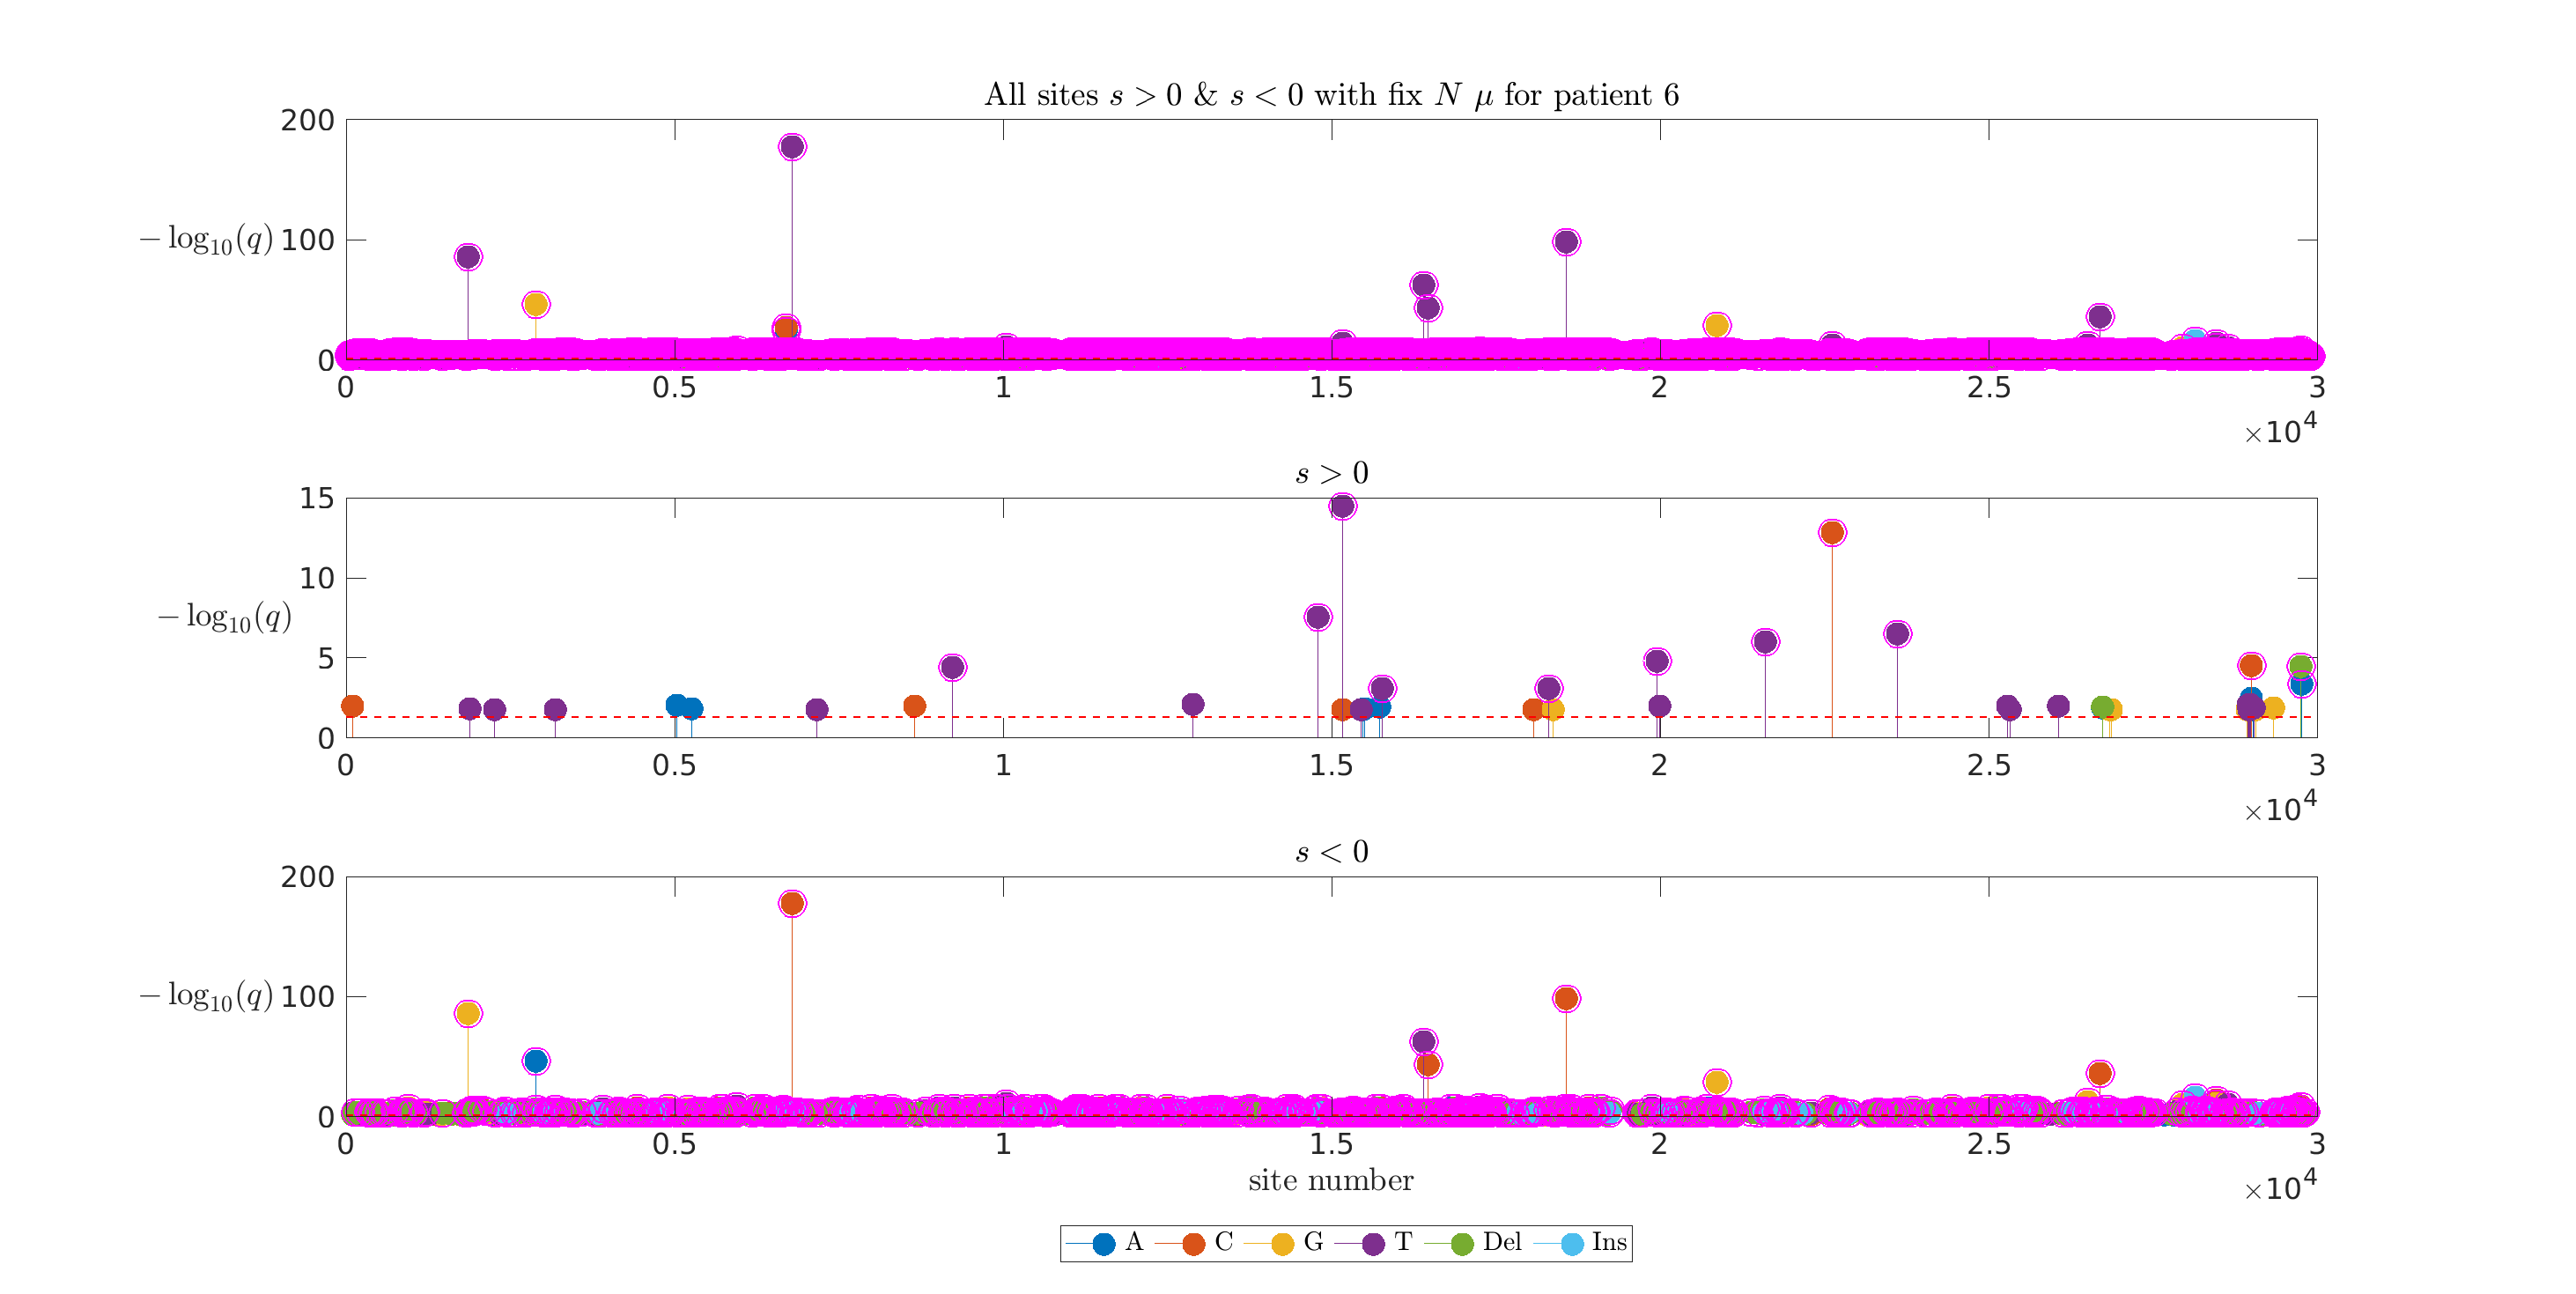
\includegraphics[height=0.45\textheight]{figures/patient/pt6/pt6_siteunder_selection_all_fixNmu.eps}
        
        \caption{Selected sites for fixing $N \mu$ in patient 6}
        \label{fig:subfig4}
    \end{subfigure}
    
    \caption{\textbf{Selection sites lollipop plot for both positive and negative selection in patien 6 for 4 constrained parameters situations}From top to bottom in each plot are the $-\log_{10}(q)$ values of all selection sites, negative selection sites and positive selection sites. The larger the value, the closer the $q-value$ of that site is to 0. All sites above the red dash line are sites greater than $-\log_{10}(\alpha=0.05)$, indicating that they are significantly selected under the hypothesis test. All the sites with pink circles outside indicate the selected sites that have passed the screening of the BH method, and the sites screened by the BH method are also more stringent.}
    \label{fig:four_subfigs}
\end{figure}

\begin{figure}[H]
    \centering
    \hspace{-6cm}
    \vspace{-4cm}
    \begin{subfigure}{0.7\textwidth}
    \hspace{-2.5cm}
            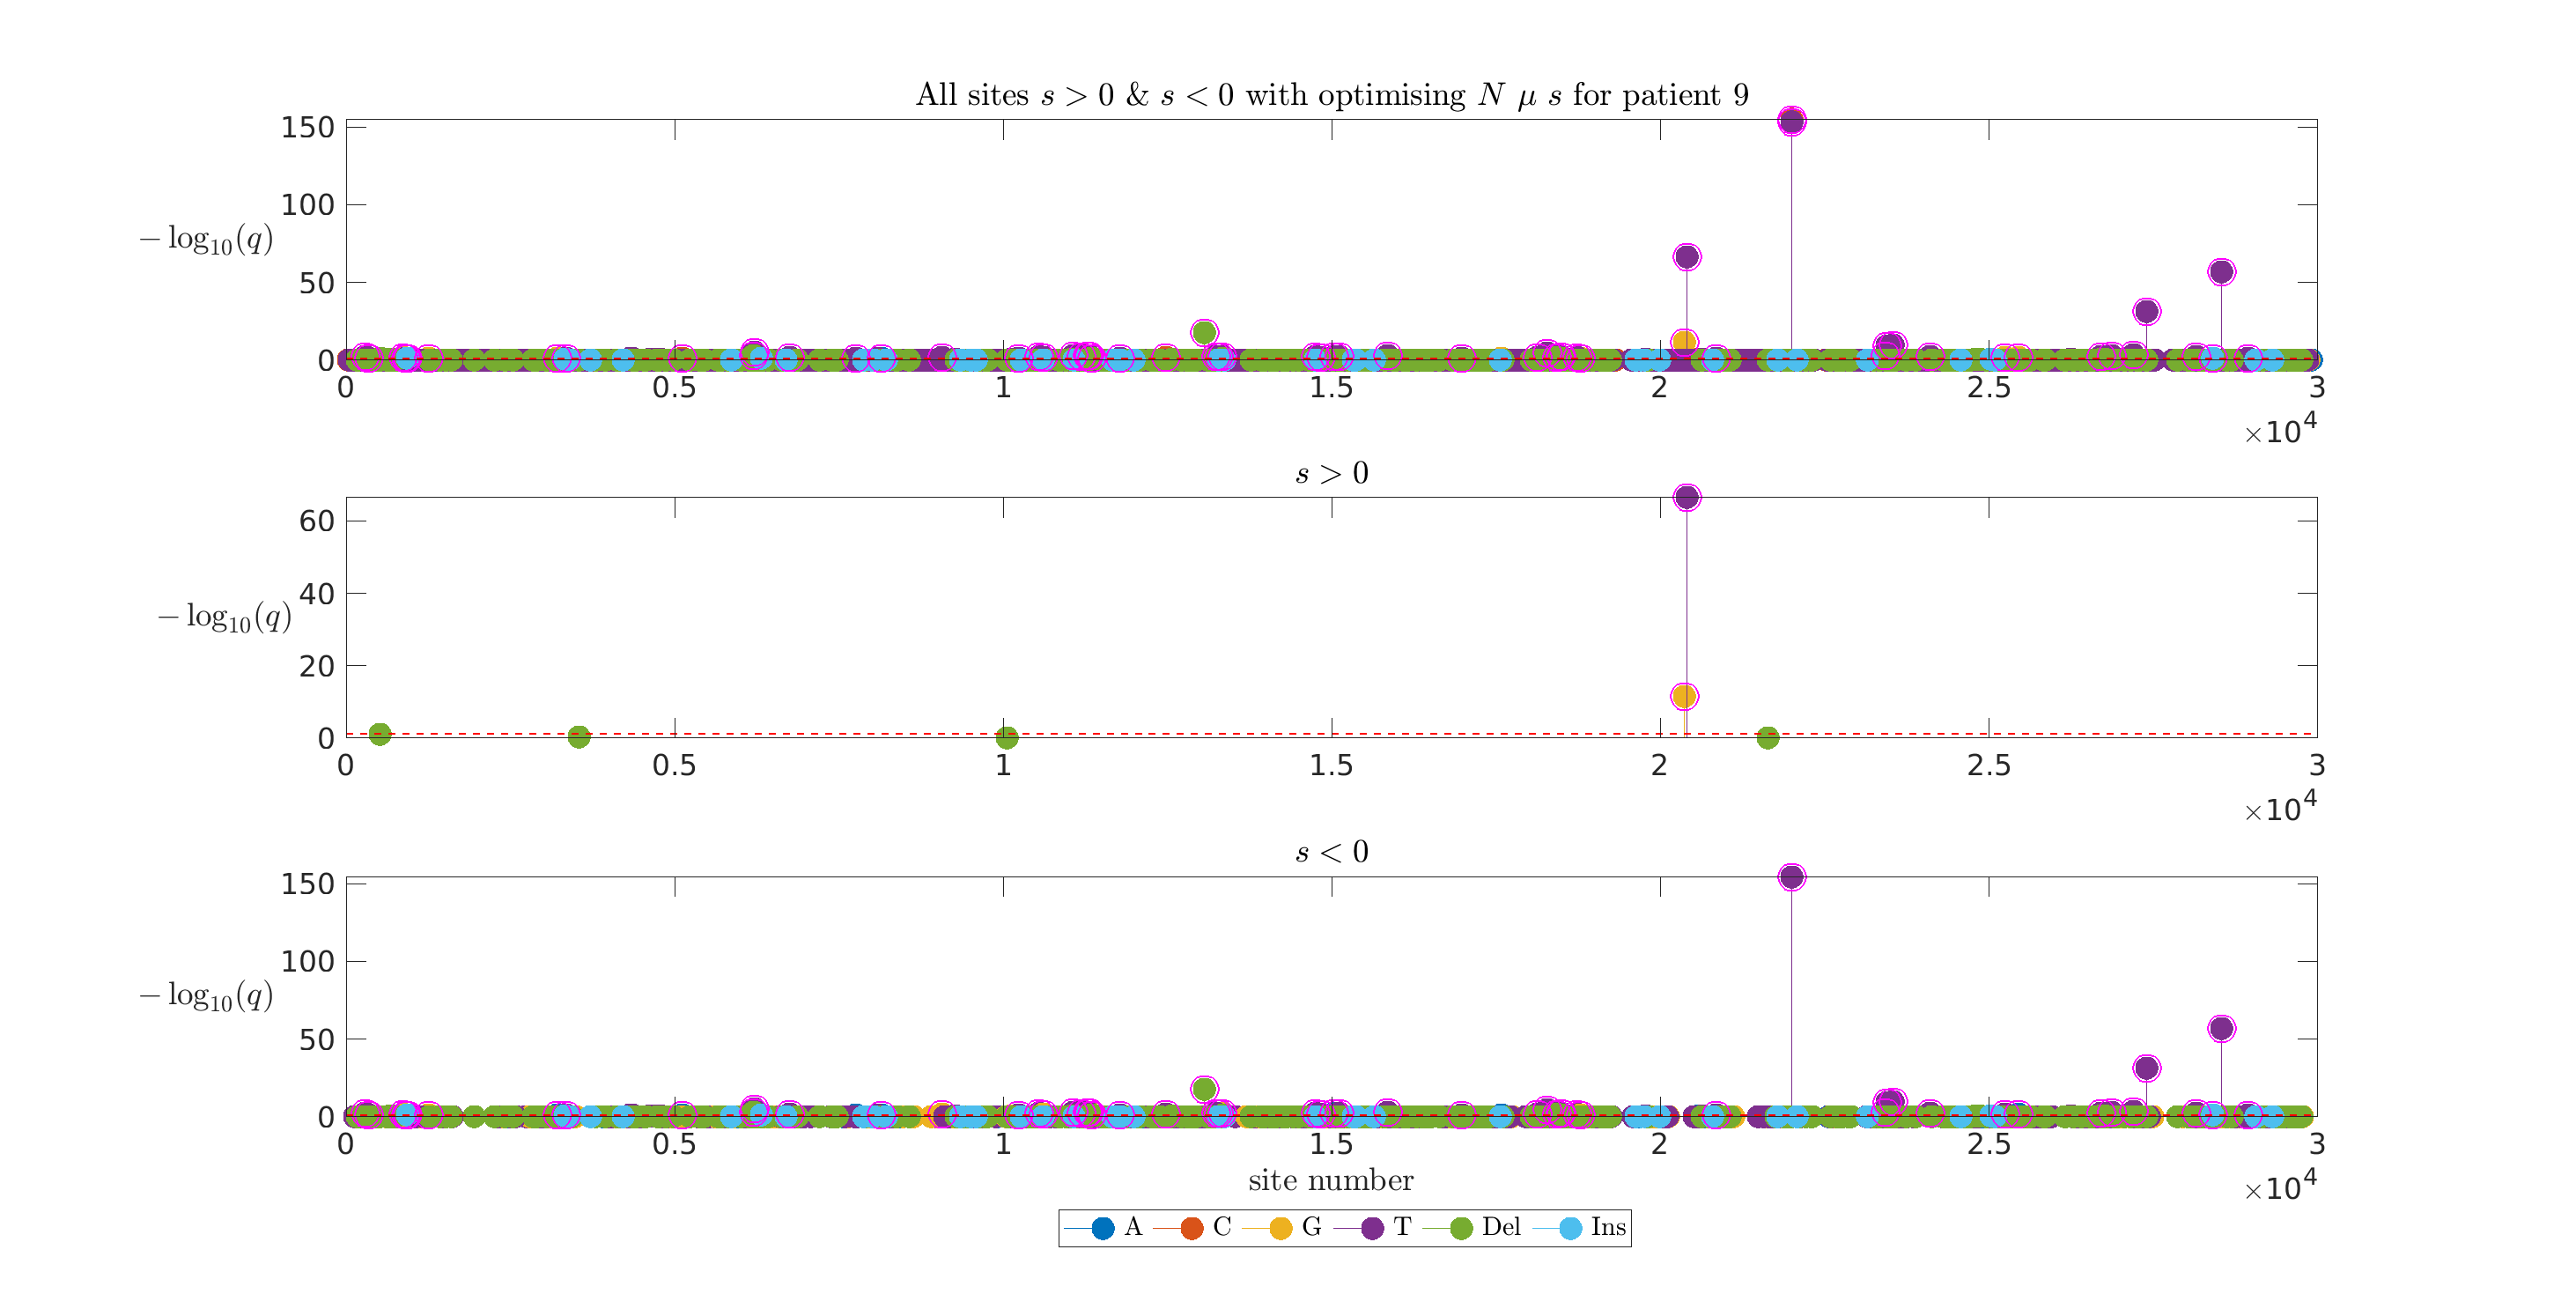
\includegraphics[height=0.5\textheight]{figures/patient/pt9/pt9_site_all_opt.eps}
        
        \caption{Selected site for optimising $N\ \mu\ s$ in patient 9}
        \label{fig:subfig1}
    \end{subfigure}
\end{figure}
\vspace{4cm}
\begin{figure}[H]
    \ContinuedFloat
    \begin{subfigure}{0.7\textwidth}
    
    \hspace{-2.5cm}
            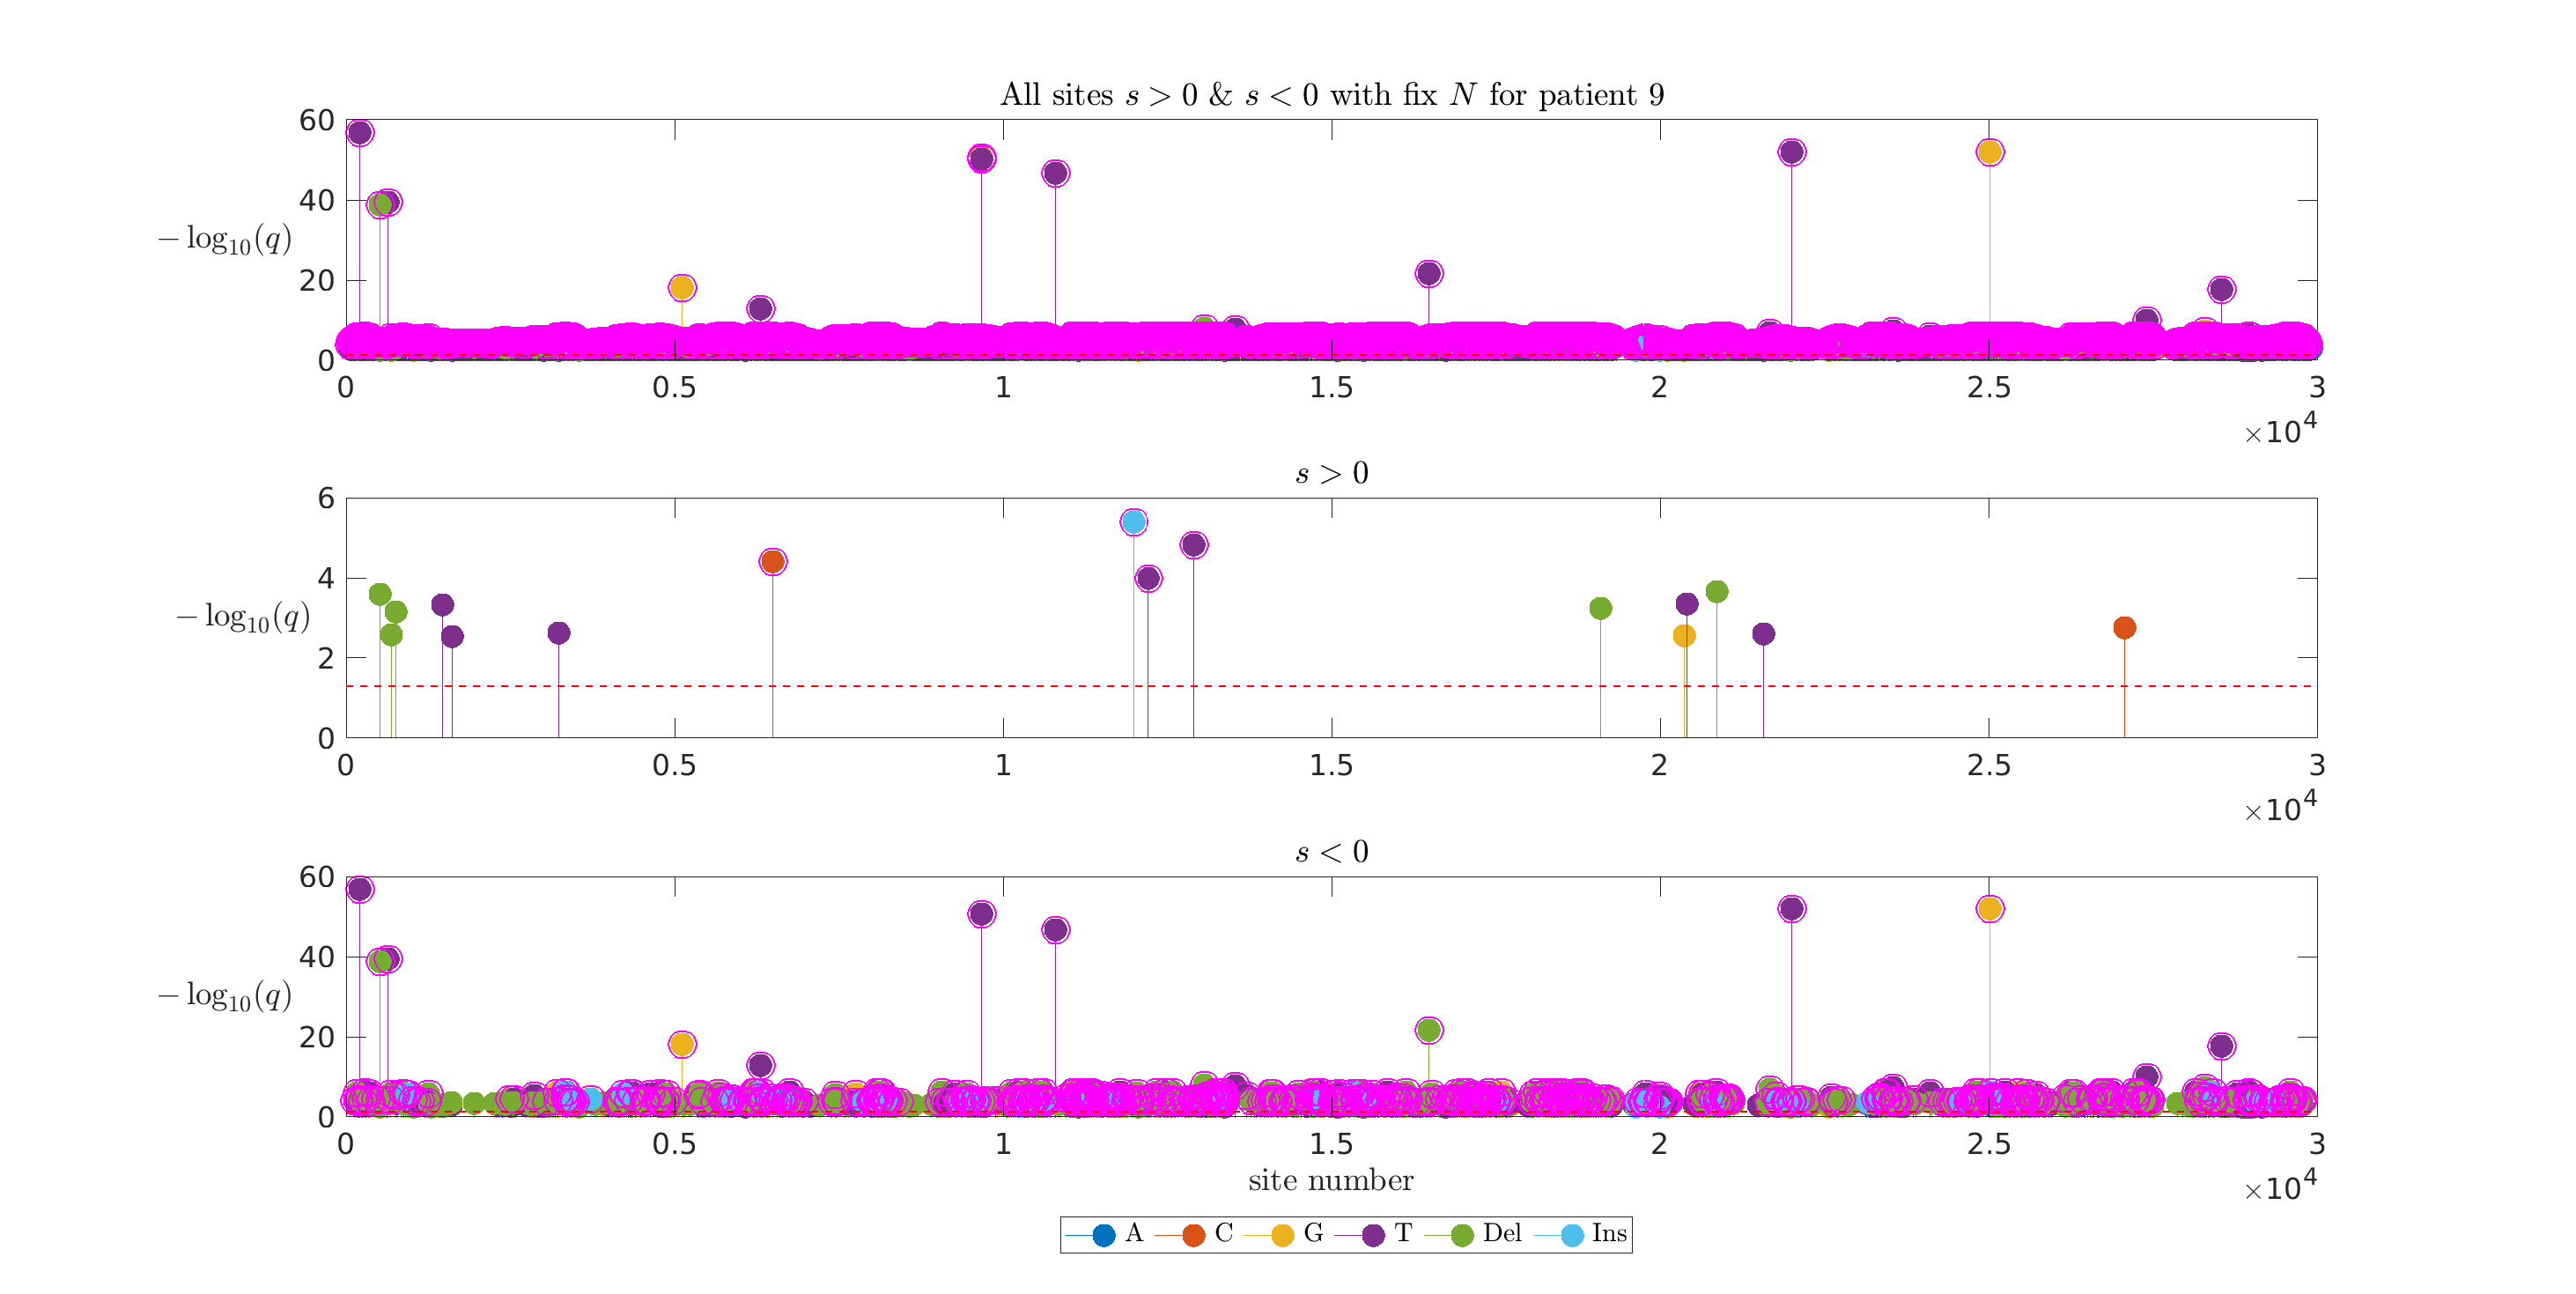
\includegraphics[height=0.5\textheight]{figures/patient/pt9/pt9_siteunder_selection_all_fixN.eps}
       
        \caption{Selected site for fixing $N$ in patient 9}
        \label{fig:subfig2}
    \end{subfigure}
    \end{figure}

\begin{figure}[H]
    \ContinuedFloat
    
    
    \begin{subfigure}{0.7\textwidth}
    \hspace{-2.5cm}
            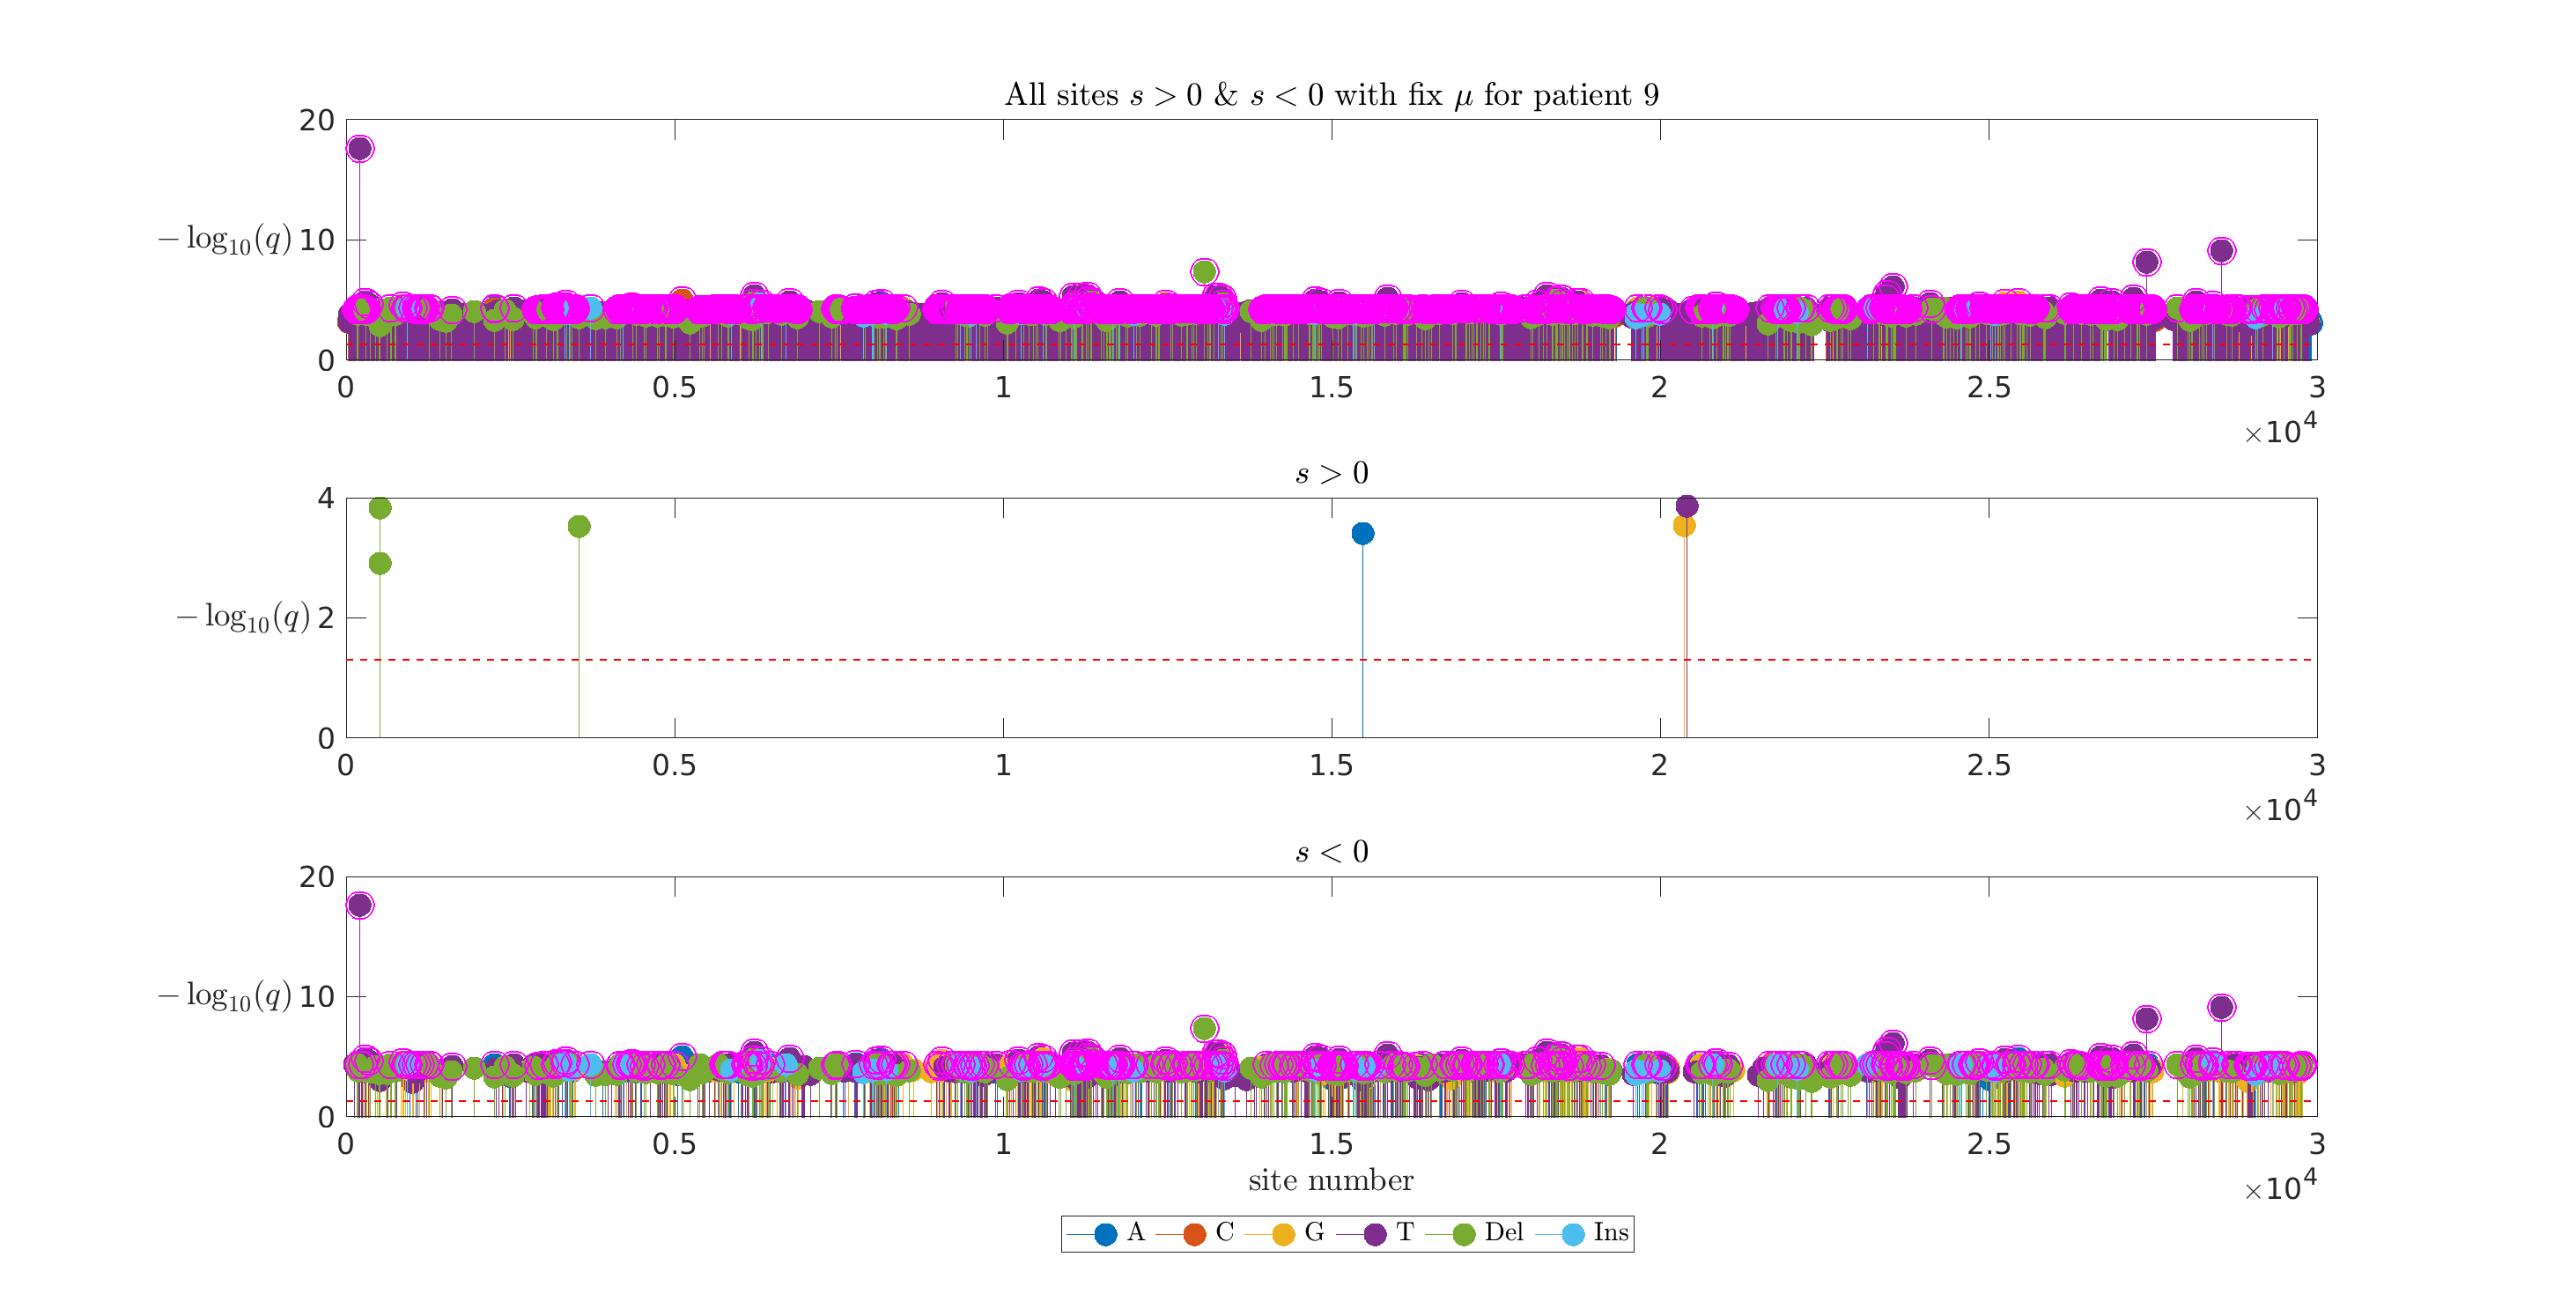
\includegraphics[height=0.5\textheight]{figures/patient/pt9/pt9_siteunder_selection_all_fixmu.eps}
        
        \caption{Selected site for fixing $\mu$ in patient 9}
        \label{fig:subfig3}
    \end{subfigure}
        \end{figure}

\begin{figure}[H]
    \ContinuedFloat

    
    \begin{subfigure}{0.7\textwidth}
    
    
        \hspace{-2.5cm}
            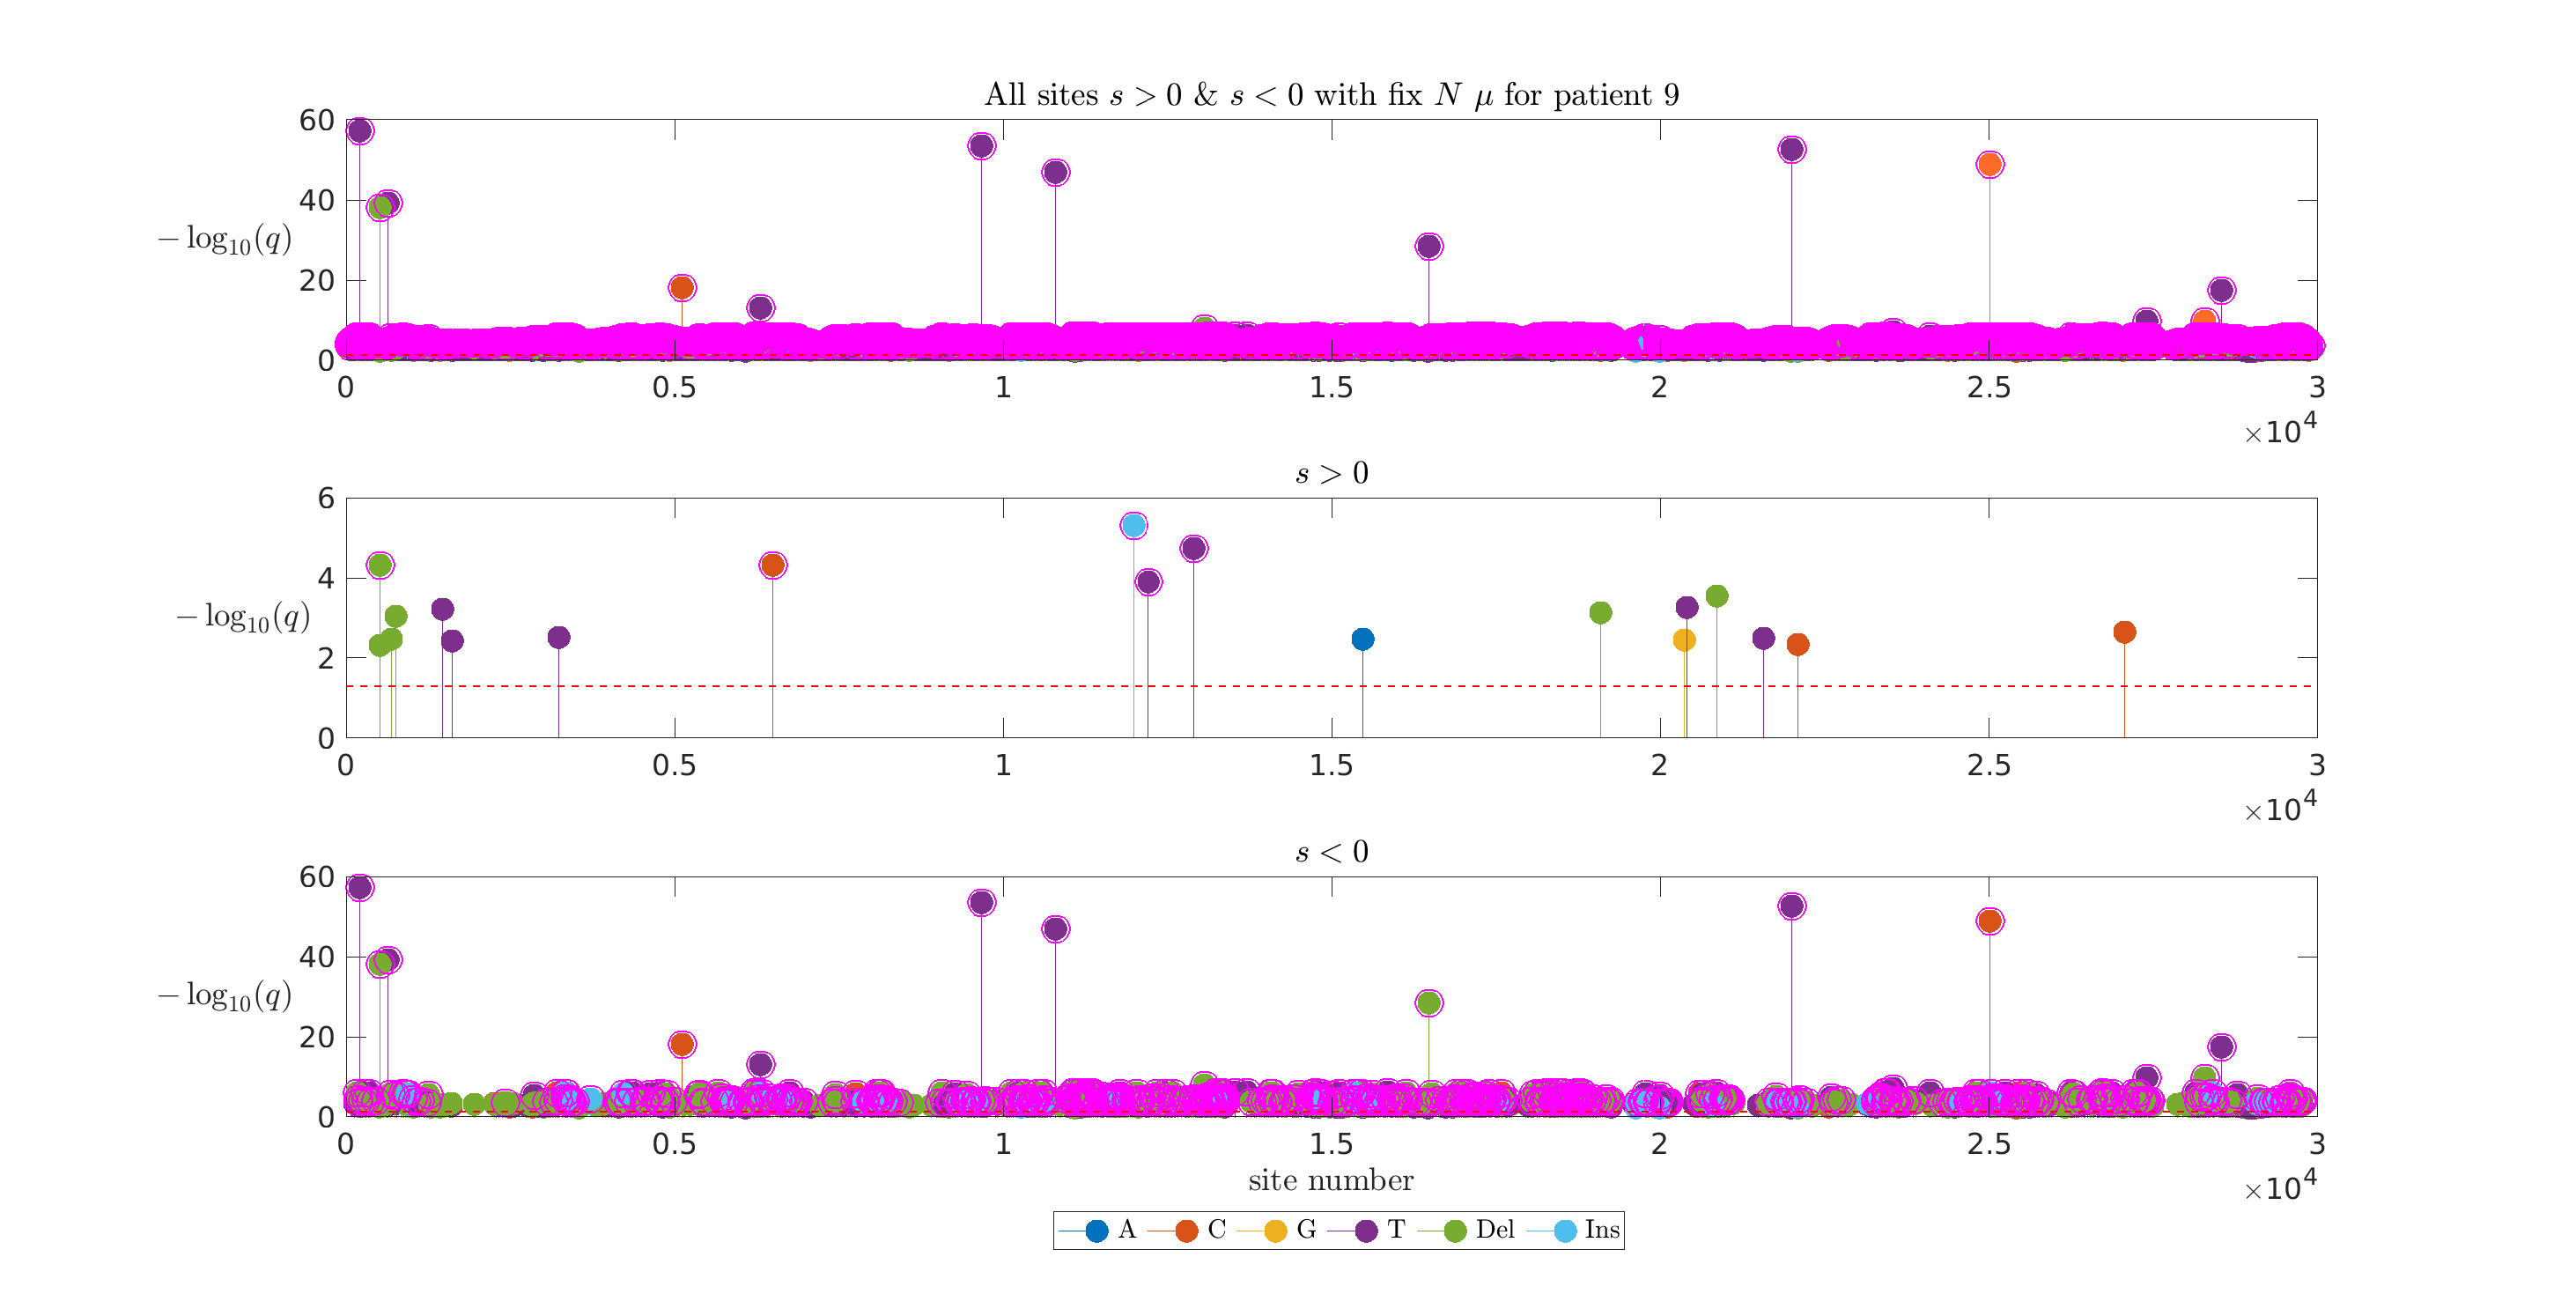
\includegraphics[height=0.45\textheight]{figures/patient/pt9/pt9_siteunder_selection_all_fixNmu.eps}
        
        \caption{Selected sites for fixing $N \mu$ in patient 9}
        \label{fig:subfig4}
    \end{subfigure}
    
    \caption{\textbf{Selection sites lollipop plot for both positive and negative selection in patien 9 for 4 constrained parameters situations}From top to bottom in each plot are the $-\log_{10}(q)$ values of all selection sites, negative selection sites and positive selection sites. The larger the value, the closer the $q-value$ of that site is to 0. All sites above the red dash line are sites greater than $-\log_{10}(\alpha=0.05)$, indicating that they are significantly selected under the hypothesis test. All the sites with pink circles outside indicate the selected sites that have passed the screening of the BH method, and the sites screened by the BH method are also more stringent.}
    \label{fig:four_subfigs}
\end{figure}


%**********************************************%
\newpage
\section{Discussion}
Independently detecting whether a locus is under selection through a frequency change time series of genes can be a viable approach, especially for segregating variations within a single population. This is basically based on the analysis of statistical methods to make a decision. Therefore, the accuracy of decision has become the primary criterion for evaluating the method. This brings us to first explore the accuracy of parameter estimation by using maximum likelihood estimation under four fixed parameter cases through single site simulations for both positive selection and negative selection.\\

There are four cases of fixing parameters are considered: Optimising $N\ \mu\ s$, fixing $N$ to optimise $\mu\ s$, fixing $\mu$ to optimise $N\ s$, fixing $N \mu$ to optimise $s$. In the case of different fixed parameters, the optimal way seems to fix the population ($N$ size and mutation rate ($\mu$). Among the four cases, when their changing trends are mostly the same, fixing $N\ \mu$ can have the best result of detecting selection among 4 cases.\\

For the estimation of $s$, under positive selection mostly has lower errors than under negative selection. This shows that estimation under the positive is more accurate than the negative selection.  This may be due to the difference in frequency change conditions under positive and negative selection. We mentioned in the Method that under strong positive selection ($2Ns>>1$), there is a situation where the mutant is established (100 generations under our setting) and reaches a fixed position after an average of 261 generations, so under the same parameter setting and the same actual frequency , every simulation of positive selection shows roughly the same changing frequency trend (eventually reaches fixation); However, under negative selection, we only mention the existence of mutation and selection balance, and the change trend during the period is not yet known, so there may be different results for each simulation , which may lead to more accurate estimation of the parameters by forward selection.\\

For the estimation of $N$, under positive selection, the $N$ error has a certain $\Delta t$ as the inflection point (20 for optimising the three parameters, 50 for fixing $\mu$). The accuracy increases at low sampling intervals and decreases at high sampling intervals. And when the starting frequency is greater than the established frequency ($x^*=1/2Ns=0.01$), the parameter estimation error is larger than the case where the starting frequency is lower than the established frequency. This should be related to the reason that the sites that reach the establishment frequency and the sites that do not reach the establishment frequency will reach fixation at different times. As the frequency change situation is different before the establishment and after the establishment, this may lead to the above results.\\

Under negative selection, when $\mu$ is fixed and $\Delta t=30$, overvaluation occurs. This is the opposite of the change under positive selection before this sampling interval. We suspect there is a reason for this. It may be due to the insufficient number of single site simulations that some occasional situations occur more frequently, resulting in a large error in the estimation of $\mu$. It can be found that when $\mu$ is fixed, the error is reduced a lot. In the case of optimizing the three parameters, the change of $N$ error in the first few sampling intervals is completely different from the above-mentioned fixing $\mu$. The parameters estimate in the first few sampling intervals are very approximate, and the subsequent trend is similar to the previous case.\\

For the estimation of $\mu$, the variation trend of the error of positive and negative selection is very close. In positive selection, the error gap between different initial frequencies increases with the increase of the sampling interval, which may also be related to the smaller change of the frequency change at smaller intervals, and the larger sampling interval , maybe the details of some frequency changes are ignored, so that the parameters can find the real optimal parameter in the maximum likelihood estimation.\\

It should also be noted that for the estimation of parameters $N$ and $\mu$, when $\Delta t=500, x_0=0.5$, there will be an obvious increase in the error compared with other parameter constrained cases. We suspect that this is due to the effect on the parameter estimates caused by excessively exceeding the initial frequency of the establishment frequency so that the frequency reaches fixation earlier.\\

Then, we explore the accuracy of finding selection sites is related to whether the population size and mutation rate are fixed. The simulated genome wide frequency change data is compared with two large datasets from SARS-CoV-2 intrahost patients. we demonstrate that it is more accurate under fixing $N$ and fixing $N \mu$ to detect selection sites.\\

Our calculation and analysis of the genome-wide simulated data further show that with the increase of the sampling interval, the accuracy of detection selection is also improved, and the results are more stable when the sampling time is larger, as AUC at T=10000 $\Delta t>100$ are kept at 0.8-0.9 which are higher and then in T=1000 and lower sampling interval (bouncing between 0.5-0.8).\\

There are four cases of fixing parameters are considered: Optimising $N\ \mu\ s$, fixing $N$ to optimise $\mu\ s$, fixing $\mu$ to optimise $N\ s$, fixing $N \mu$ to optimise $s$. In the case of different fixed parameters, the optimal way seems to fix the population ($N$ size and mutation rate ($\mu$). Among the four cases, when their changing trends are mostly the same, fixing $N\ \mu$ can have the best result of detecting selection among 4 cases.\\

However, both positive and negative selection are simulated during genome wide simulation, but they does not analysed separately. The two selection cases should be separated to examine the effect of the four cases of parameter constraining on different type of selection sites detection.  Also, separate positive selection and  negative selection can better align with real data, then compare the accuracy under each selection scenario.\\

Such result can also be reflected in the results of patient data. In the two groups of patient data, more significant sites were brought about by fixing $N\ \mu$. However, different from the simulated situation, the time interval for sampling and analysis in reality is often not regular. The average total generation of SARS-CoV-2 virus in the two patient data in this study are 181 and 350 generations according to gamma (2generations per day) of SARS-COV-2 \citep{markov2023evolution}, respectively, and the average sampling interval was 16 generations and 18 generations. If the two sets of data are put in the analysis of the AUC results analysed by the simulated data, patient 6 is close to sampling interval of 20 generations in the simulated data, and patient 9 is closest to the sampling interval of 50 generations. The optimal constrained parameter conditions for them is fixing $N\ \mu$. But in fact, we didn't set suitable intervals that fits to patient data. Perhaps for the real sampling interval of patients, there will be different fixed parameter selections that can make the results of screening selection sites more accurate.\\

Moreover, whether the frequency can finally be fixed is not necessarily for the diagnosed patient, it is an unknown situation, we cannot know how the frequency will change after receiving treatment, so the simulation here does not consider intercepting different frequencies to see the impact on parameter estimation. There is also no consideration of the impact of intervention of treatment on changes in virus frequency and population size, which can be considered in the simulation to more closely match the reality.\\ 

In what actually happens, there may be linkage \citep{lewontin1960evolutionary}, the genetic link between certain loci, between loci in the genome. This could lead to mutations spreading across the genome differently than expected from independent allelic models. Therefore, when performing genome-level simulations, factors such as linkage effects may need to be considered, and even more complex models may need to be used \citep{slatkin2008linkage}. These actual factors have not been well considered and involved in this simulation. It is just that the loci that have received selection are screened out through multiple hypothesis testing analysis independently.


%**********************************************%
\newpage
\section{Conclusion}
This study analysed the time series of gene frequency changes, and explored the effect and accuracy of the four fixed parameters conditions on the detection site under selection. First, through single site analysis, the influence of four fixed parameters on the accuracy of parameter estimation was evaluated, and the results were obtained that fixing $N$ and $\mu$ have more accurate parameters estimation at low sampling intervals, and the accuracy of $s$ estimation increases with sampling intervals increasing. In addition, the study also simulated the genome wide data to conduct multi-hypothesis testing to detect the selection sites. Then the gene frequency change data of SARS-CoV-2 in immunocompromised patients were used to compare with simulated data. It was found that fixing parameters $N \mu$ has a better outcomes than fixing $N$, fixing $\mu$ and optimising $N\ \mu\ s$ at same time.



\newpage
\section{Data and code availability}
Code for likelihood estimation and multi-hypothesis part and data can't be released. For the generation code of frequency simulation data based on WF model, contact the author by email to obtain permission. (https://github.com/\\chuxinyaowang/MSc$\_$project.git)


%**********************************************%
\newpage
\section{Reference list}
\bibliographystyle{agsm}


\bibliography{references}

\newpage
\section{Appendix}
\newcommand{\imageopt}{
  {/ROCopt/u1000_5.eps},
  {/ROCopt/u1000_10.eps},
  {/ROCopt/u1000_20.eps},
  {/ROCopt/u1000_50.eps},
  {/ROCopt/u10000_50.eps},
  {/ROCopt/u10000_100.eps},
  {/ROCopt/u10000_200.eps},
  {/ROCopt/u10000_500.eps},
  {/ROCopt/1000_5.eps},
  {/ROCopt/1000_10.eps},
  {/ROCopt/1000_20.eps},
  {/ROCopt/1000_50.eps},
  {/ROCopt/10000_50.eps},
  {/ROCopt/10000_100.eps},
  {/ROCopt/10000_200.eps},
  {/ROCopt/10000_500.eps},
}


\newcommand{\imagefixn}{
  {/ROCfixN/u1000_5.eps},
  {/ROCfixN/u1000_10.eps},
  {/ROCfixN/u1000_20.eps},
  {/ROCfixN/u1000_50.eps},
  {/ROCfixN/u10000_50.eps},
  {/ROCfixN/u10000_100.eps},
  {/ROCfixN/u10000_200.eps},
  {/ROCfixN/u10000_500.eps},
  {/ROCfixN/1000_5.eps},
  {/ROCfixN/1000_10.eps},
  {/ROCfixN/1000_20.eps},
  {/ROCfixN/1000_50.eps},
  {/ROCfixN/10000_50.eps},
  {/ROCfixN/10000_100.eps},
  {/ROCfixN/10000_200.eps},
  {/ROCfixN/10000_500.eps},
}

\newcommand{\imagefixmu}{
  {/ROCfixmu/u1000_5.eps},
  {/ROCfixmu/u1000_10.eps},
  {/ROCfixmu/u1000_20.eps},
  {/ROCfixmu/u1000_50.eps},
  {/ROCfixmu/u10000_50.eps},
  {/ROCfixmu/u10000_100.eps},
  {/ROCfixmu/u10000_200.eps},
  {/ROCfixmu/u10000_500.eps},
  {/ROCfixmu/1000_5.eps},
  {/ROCfixmu/1000_10.eps},
  {/ROCfixmu/1000_20.eps},
  {/ROCfixmu/1000_50.eps},
  {/ROCfixmu/10000_50.eps},
  {/ROCfixmu/10000_100.eps},
  {/ROCfixmu/10000_200.eps},
  {/ROCfixmu/10000_500.eps},
}


\newcommand{\imagefixnmu}{
  {/ROCfixNmu/u1000_5.eps},
  {/ROCfixNmu/u1000_10.eps},
  {/ROCfixNmu/u1000_20.eps},
  {/ROCfixNmu/u1000_50.eps},
  {/ROCfixNmu/u10000_50.eps},
  {/ROCfixNmu/u10000_100.eps},
  {/ROCfixNmu/u10000_200.eps},
  {/ROCfixNmu/u10000_500.eps},
  {/ROCfixNmu/1000_5.eps},
  {/ROCfixNmu/1000_10.eps},
  {/ROCfixNmu/1000_20.eps},
  {/ROCfixNmu/1000_50.eps},
  {/ROCfixNmu/10000_50.eps},
  {/ROCfixNmu/10000_100.eps},
  {/ROCfixNmu/10000_200.eps},
  {/ROCfixNmu/10000_500.eps},
}



\newcommand{\imagens}{
  {/appendix/pt6_Ne_vs_s.eps},
  {/appendix/pt6_fixN_Ne_vs_s.eps},
  {/appendix/pt6_fixmu_Ne_vs_s.eps},
  {/appendix/pt6_fixNmu_Ne_vs_s.eps},
  {/appendix/pt9_Ne_vs_s.eps},
  {/appendix/pt9_fixN_Ne_vs_s.eps},
  {/appendix/pt9_fixmu_Ne_vs_s.eps},
  {/appendix/pt9_fixNmu_Ne_vs_s.eps},
}

\subsection{ROC plots for optimising $N$ $\mu$ $s$ with and without sampling in genome-wide simulation}
\foreach \image in \imageopt {
  \begin{figure}[htbp]
    \centering
    \includegraphics[width=1\linewidth]{\image}
    \label{fig:\image}
  \end{figure}
}
\newpage
\subsection{ROC plots for fixing $N$ with and without sampling in genome-wide simulation}
\foreach \image in \imagefixn {
  \begin{figure}[htbp]
    \centering
    \includegraphics[width=1\linewidth]{\image}
    \label{fig:\image}
  \end{figure}
}
\vfill

\newpage
\subsection{ROC plots for fixing $\mu$ with and without sampling in genome-wide simulation}
\foreach \image in \imagefixmu {
  \begin{figure}[htbp]
    \centering
    \includegraphics[width=1\linewidth]{\image}
    \label{fig:\image}
  \end{figure}
}

\newpage
\subsection{ROC plots for fixing $N\ \mu$ with and without sampling in genome-wide simulation}
\foreach \image in \imagefixnmu {
  \begin{figure}[htbp]
    \centering
    \includegraphics[width=1\linewidth]{\image}
    \label{fig:\image}
  \end{figure}
}

\newpage
\subsection{Scatter plots for $N$ vs. $\mu$ for patient 6 and 9 under 4 parameters constrained conditions}
\textbf{From top to bottom are:\\ Optimising $N\ \mu\ s$,\\ Fixing $N$,\\ Fixing $\mu$,\\ Fixing $N\ \mu$.\\
First four figures are from patient 6, then patient 9}
\foreach \image in \imagens {
  \begin{figure}[htbp]
    \centering
    \includegraphics[width=1\linewidth]{\image}
    \label{fig:\image}
  \end{figure}
}

\end{document}